\documentclass[a4paper,12pt,numbers=noenddot]{report}

\usepackage{polski}
\usepackage[utf8]{inputenc}
\usepackage{graphicx}
\usepackage{cite}
\usepackage{float}
\usepackage{url} 
\usepackage{hyperref}
\usepackage{amsmath}
\usepackage{gensymb}
\usepackage{pdfpages}
\usepackage[nottoc,numbib]{tocbibind}
\usepackage{etoolbox}
\usepackage{enumitem}
 
\usepackage{multirow}
\usepackage{bigstrut}
\usepackage{rotating}
\usepackage{xcolor}
\usepackage{colortbl}

\usepackage{titlesec, blindtext, color}

\titleformat{\chapter}[hang]{\Huge\bfseries}{\thechapter{. }}{0pt}{\Huge\bfseries}


\usepackage[
  inner = 3cm,
  outer = 2.5cm,
  top = 2.5cm,
  bottom = 2.5cm,
]{geometry}


\title{TYTUŁ pracy}
\date{\today}
\author{Hubert Marcinkowski}

\begin{document}
	\nocite{*}
	\pagenumbering{gobble}
	%\maketitle
	
\includepdf{first_page.pdf}

	\newpage
	\pagenumbering{arabic}
	\tableofcontents
	\newpage
	%\setcitestyle{square}	
%CHAPTER_______________________________________________________________________________________WSTĘP_______	
\chapter{Wstęp}
Branża gier wideo jest jedną z najprężniej rozwijających się gałęzi gospodarki. Około 2 mld graczy generuje rocznie ponad 100 mld przychodu. Największą tego część w roku 2017 zarejestrowano dla gier mobilnych. Składają się one na 32\% całego rynku, gdzie jeszcze rok wcześniej było to o trzy procent mniej. Do roku 2020 przewidywane jest że gry mobilne stanowić będą połowę wszystkich przychodów przemysłu gier \cite{art_Market2017}. 

W tak dynamicznie rozwijającym się środowisku coraz trudniej stworzyć jest produkt, który zauważony zostanie przez konsumentów. Twórcy prześcigają się zatem w tworzeniu coraz to lepszych produktów, które wyróżnić się mogą jakimiś określonymi cechami, które w przypadku gier mogą być powierzchowne jak i bardziej złożone. D tej drugiej kategorii zaliczać może się chociażby to, jakie odczucia wywołuje w użytkowniku korzystanie z danej aplikacji. Istnieje zawsze szansa, że wynikiem długiego procesu tworzenia może się okazać produkt, który nie spełnia oczekiwań użytkowników. Poszukiwany zatem jest pewien zestaw reguł, który już nawet na procesie projektowania gry pozwoliłby na określenie, czy ma ona szansę na osiągnięcie sukcesu. 

Powstało wiele publikacji, które mają na celu ścisłe przedstawienie heurystyk, które to powinny spełniać aplikacje. Dotyczą one wiele aspektów tworzenia tego typu produktów, między innymi \textit{użyteczności}. Podzbiorem tej kolekcji są prace naukowe, które usiłują znaleźć takie zasady dla bardziej sprecyzowanego zakresu, jakim są gry mobilne. Pod uwagę w procesie tworzenia trzeba bowiem w nich brać pod uwagę dużo więcej składowych, jak na przykład przyjemność, jaką gracze powinni odczuć w procesie użytkowania aplikacji czy charakterystyczny kontekst użycia. Wielu ekspertów podjęło się prób przedstawienia heurystyk, które często wykorzystywane są w dzisiejszych produkcjach.

Pojawia się jednak pytanie jak bardzo stosowanie się do tych ściśle określonych reguł wspomóc może projektantów w stworzeniu gry, której mechaniki będą dla graczy zrozumiałe. Nie jest wymagane by zawsze one miały odniesienie w rzeczywistości. Czasem wykonywanie abstrakcyjnych akcji może być zrozumiane przez użytkowników szybciej, niż to czego oczekuje od nich aplikacja, w której zadaniem jest wykonanie czegoś, co robią oni w życiu codziennym. W pracy tej przedstawione zostanie właśnie takie badanie, które na celu miało zweryfikować, czy gry spełniające wybrane heurystyki są czytelniejsze pod względem przedstawiania swoich zasad. 

%CHAPTER__________________________________________________________________________CEL, ZAŁOŻENIA, ZAKRES__
\chapter{Cel, założenia oraz zakres pracy}
Celem tej pracy było zbadanie wpływu określonych heurystyk dotyczących projektowania interfejsów na jakość przyswajania nowych mechanik gry mobilnej, która z nich korzysta. Badaniu podane zostały zasady, które odnoszą się do użyteczności tworzonych aplikacji.

Ustalanie heurystyk ma na celu określenie wytycznych, za pomocą których deweloperzy gier są już w~stanie określić, czy przygotowywany przez nich projekt ma szansę spodobać się odbiorcom. Spodziewać się można, że przy porównaniu dwóch aplikacji zajmujących się jednym zagadnieniem, gdzie jedna z nich spełnia większą ilość heurystyk użyteczności z zadanego zakresu to poprawnie wykonane testy wykażą, że jest ona bardziej użyteczna. Cecha ta definiuje między innymi stopień wydajności z jaką użytkownik jest w~stanie zrozumieć prezentowane mu przez aplikację treści. Oznaczać to może, że badając, jakie heurystyki spełnia dana gra, można oszacować jak zrozumiała mogła by ona być dla jej docelowego użytkownika. Przetestowaniu podlegać ma zrozumienie mechanik gry, czyli to jak sprawnie gracze są w stanie wykorzystywać panujące w niej reguły do wykonywania założonych celów.\\
Bazując na tych założeniach, praca ta ma na celu sprawdzenie następujących hipotez:

\begin{enumerate}
\item Zrozumienie mechanik gry mobilnej przychodzi użytkownikom łatwiej dla gier spełniających więcej heurystyk użyteczności.
\item Użytkownicy popełniają mniej błędów w~wypadku gier spełniających więcej heurystyk użyteczności
\item Użytkownicy grający w~grę spełniającą mniej heurystyk użyteczności osiągają gorsze wyniki od tych, którzy grają w~wersję spełniającą ich więcej.
\end{enumerate}

W celu ich przetestowania przeprowadzone zostało doświadczenie, w~którym za pomocą testów rozgrywki (ang. \textit{playtesting}) badane były cztery wersje tej samej gry mobilnej w~różnym stopniu spełniające wybrane heurystyki odnoszące się do użyteczności gier. Dane z każdego testu były zapisywane automatycznie przez aplikację do pliku a~następnie zostały one przeniesione do arkusza kalkulacyjnego, gdzie wykonano ich analizę. Wyniki opracowano i~przedstawiono w~postaci czytelnych dla osób postronnych wykresów.


%CHAPTER_______________________________________________________________________________WYJAŚNIANIE POJĘĆ___
\chapter{Grywalność w~grach mobilnych}
Przed rozpoczęciem analizy kluczowym zdaje się dokładne wyjaśnienie podstawowych pojęć, jakie wykorzystywane są w~tej pracy. w~tym rozdziale wyjaśnione zostanie co definiowane jest jako mechanika gry, doświadczenie użytkownika, czym jest grywalność i~użyteczność a~także przybliżone będą ograniczenia i~przeszkody związane z rozgrywką na urządzeniach mobilnych.

\section{Heurystyka}
Mianem heurystyk określa się zestaw zasad, których przeznaczeniem jest zwiększenie prawdopodobieństwo rozwiązania określonego problemu \cite{art_WithHeuristic}. Służą one jako pomoc przy rozwiązywaniu problemów przy pomocy eksperymentalnych metod. w~przypadku metod mierzących użyteczność skupiają się one na zagadnieniach, które sprawiają problemy podczas interakcji\cite{art_Nielsen}\cite{art_evaluatingPlayabilityMG}. 

\section{Mechanika gry}
Mechaniki gry zdefiniować można jako zestaw reguł zaprojektowanych w~celu zapewnienia użytkownikowi interakcji ze stanem gry. Zestawienie różnych mechanik rozgrywki określa stopień skomplikowania jak również ilość akcji, których wykonanie wymagane jest od użytkownika. Innymi słowy określić je można jako zbiór zasad, które pozwalają graczowi na postęp w~przestrzeni gry. \cite{online_GameMechanics}

\section{Doświadczenie użytkownika}

Pojęciem doświadczenia użytkownika (\textit{User Experience} - UX) opisuje się całość wrażeń, z którymi spotyka się osoba podczas procesu użytkowania określonego produktu bądź usługi. Pod tym pojęciem zawierają się wszelkie aspekty interakcji człowiek-komputer oraz wrażenia osoby użytkującej dotyczące takich aspektów systemu jak na przykład łatwość w~użyciu czy wydajność. Wyróżnia się trzy czynniki wpływające na UX: system, użytkownik oraz kontekst użycia. \cite{online_UXDef}
Celem projektowania dobrego UX jest osiągnięcie jak największej produktywności przy pracy z systemem, czyli innymi słowy - spełnienie oczekiwań użytkownika. Ważnym aspektem poprawnie zaprojektowanego UX jest również to, by korzystanie z przygotowanego systemu było przyjemne i~proste. Projektowania doświadczenia użytkownika się między innymi w~celu wyeliminowania błędów interfejsów, czy zmniejszenia ilości operacji, które wymagane są do wykonania określonego zadania.
\cite{art_UserExperience}

\section{Użyteczność}
Użyteczność definiowana jest jako podatność danej aplikacji do bycia używaną przez ludzi prosto i~wydajnie\cite{art_Usability}. Jest to swojego rodzaju miara pozwalająca na określenie stopnia, w~jakim dany produkt może być zrozumiany i~wykorzystywany. Określa ona również jak bardzo aplikacja jest zachęcająca dla użytkowników, którzy jej używają w~określonym środowisku. \cite{art_evaluationOfMGevaluationSystem} 
\\
Można wyróżnić siedem podstawowych czynników użyteczności: \cite{art_UsabilityEvaluationSystematicReview}
\begin{enumerate}
\item Bezmyślność (ang. \textit{learnability}) - określa jak łatwo użytkownik jest w~stanie wykonać postawione mu przez grę zadanie za pierwszym podejściem oraz jak szybko jest w~stanie polepszyć uzyskany wynik.
\item Wydajność (ang. \textit{efficiency}) - definiuje czas, jaki potrzebny jest doświadczonemu użytkownikowi na wykonanie zadania.
\item Zapamiętywanie (ang. \textit{memorability}) - miara oznaczająca łatwość, z jaką użytkownik potrafi wrócić do gry po pewnej przerwie.
\item Błędy (ang. \textit{errors}) - ilość błędów gry, jakie użytkownik popełnia w~trakcie rozgrywki.
\item Satysfakcja użytkownika (ang. \textit{user satisfaction}) - określa nastawienie użytkownika do gry
\item Prostota (ang. \textit{simplicity}) - stopień swobody z jakim wykonywać można zadania w~grze. Odnosi się zwykle do nawigacji w~różnego rodzaju ekranach menu.
\item Czytelność (ang. \textit{readability}) - określa jak łatwo użytkownik jest w~stanie zrozumieć zawartość gry.
\end{enumerate}

Wyróżnia się dwie główne metodologie mierzenia użyteczności: testowanie poprzez rozgrywkę (ang. \textit{play-testing}) oraz opinie ekspertów (ang. \textit{expert review}).

\subsection{Mierzenie użyteczności}
Testowanie poprzez rozgrywkę zakłada, iż testowanie odbywa się przez osoby z grupy docelowej tworzonego produktu\cite{art_evaluatingPlayabilityMG}. Wchodzą oni w~interakcję z aplikacją a~ich zachowanie i~wrażenia z rozgrywki są zbierane przez samą grę lub przez obserwujących ich badaczy. Metoda ta pozwala na bezpośrednie zaobserwowanie przez deweloperów w~jaki sposób gracze wykonują polecenia, które przekazywane im są za pośrednictwem aplikacji.
Zauważyć jednak należy wiele przeszkód, które nie pozwalają na określenie tego sposobu sprawdzania użyteczności jako bardzo przystępnego. Przygotowanie odpowiedniego środowiska do przeprowadzenia badania niejednokrotnie może wiązać się z dużymi nakładami pieniężnymi jak i~czasowymi. Testowanie przez graczy spoza zespołu deweloperskiego nie pozwala na uzyskanie wymiernych wyników do czasu, aż dostępny jest działający prototyp aplikacji. Musi on zwykle być wycinkiem zawierającym wszelkie właściwości, którymi cechować się ma finalna wersja gry. Problem zwiększa się w~przypadku, gdy podczas takich testów na jaw wychodzą błędy związane z grywalnością produktu. Próba ich naprawy nierzadko oznaczać może konieczność wprowadzenia poważnych zmian w~projekcie, co z kolei prowadzi do poniesienia dużych kosztów przez deweloperów. Zignorowanie tych problemów również jest ryzykowne, gdyż istnieje szansa na to, iż mogą one wpłynąć negatywnie na wrażenia związane z rozgrywką \cite{art_evaluationOfMG}.

Z tego też powodu przez wielu badaczy testowanie za pomocą opinii ekspertów jest dużo bezpieczniejszym podejściem \cite{art_UsabilityTestingComp}. w~tym wypadku rzadko zdarza się, by użytkownicy z grupy docelowej brali udział w~badaniu. Testerami jest tu dwóch lub więcej ekspertów biegłych w~dziedzinie użyteczności aplikacji \cite{art_Nielsen}. Zwykle zakresy ich ekspertyz są zbiorami jak najbardziej rozłącznymi tak, by uzyskać jak największy obszar oceny. Przeprowadzają oni niezależne testy w~oparciu o ogólnie przyjęte heurystyki i~następnie porównując swoje notatki podejmują finalną decyzję odnośnie danej aplikacji.
Dużą zaletą tej metody jest szybkość, z jaką otrzymać można pełną ocenę użyteczności gry. Eksperci dysponując dużym zakresem wiedzy w~sprawdzanej dziedzinie są w~stanie przeprowadzić pełną ewaluację w~zaledwie kilka godzin używania zarówno funkcjonalnych prototypów jak i~takich, które w~małym stopniu odwzorowują finalny produkt (papierowe makiety, koncepty czy nawet same opisy interakcji). 

Wybór metody, którą należy obrać do analizy często zależne jest od czynników takich jak ilość czasu i~pieniędzy, jakie można zainwestować w~proces testowania użyteczności. w~wypadku, gdy niedobór środków, które można na taką ocenę przeznaczyć jest czynnikiem pomijalnym najlepszym rozwiązaniem jest hybryda tych rodzajów badań. Pozwala to na połączenie ich zalet jednocześnie minimalizując ich wady.

\section{Grywalność}
Grywalność określić można jako zestaw własności, które opisują doświadczenie gracza (ang. \textit{Player Experience}) przy użyciu określonego systemu growego, którego głównym celem jest zapewnienie rozrywki poprzez jego użytkowanie zgodnie z jego przeznaczeniem. \cite{art_Playability} Odnosi się do jakości samej gry. Jest to pojęcie często używane zarówno w~procesach projektowania jak i~analizy gier pod względem ich reguł, mechanik czy zadań stawianych przez nie graczom. Na grywalność wpływa bardzo wiele czynników związanych z samą rozgrywką, jak na przykład responsywność na akcje gracza czy intensywność interakcji.
Grywalność składa się z trzech komponentów: podstawowych mechanik (zasady oraz zadania, które użytkownik ma wykonać), narracji oraz interaktywności (zestaw elementów, które są widoczne dla gracza i~z którymi może wejść w~interakcję w~przestrzeni gry). \cite{art_UserExperience}

Jak można zauważyć, pojęcie grywalności jest ściśle powiązane z użytecznością. Zaznaczyć jednak należy, że w~kontekście gier, jest ono dużo dokładniejsze. Mierzy ono nie tylko jak dobrze gracz jest w~stanie wykonywać zadania, ale również to, czy odczuwa w~trakcie wykonywania tych operacji przyjemność. Aspekty miary, jaką jest grywalność nie są ściśle określone dla każdej gry. Oznacza to, że w~zależności od gatunku do jakiego przypisana jest dana aplikacja, przypisać można różne wagi poszczególnym jej aspektom.

Zarówno jak w~przypadku użyteczności, wyróżnić można siedem czynników charakteryzujących grywalność:

\begin{enumerate}
\item Efektywność - czas i~środki, jakie potrzebne są, by zaoferować graczom przyjemne doświadczenia z wykonywania zadań postawionych przez grę.
\item Bezmyślność (ang. \textit{learnability}) - stopień w~jakim gracz jest w~stanie zrozumieć i~nauczyć się systemów i~mechanik gry. Zauważyć należy, że w~przypadku gier nie zawsze wskazane jest, by gracze zrozumieli wszystkie zasady w~nich panujące. Niekiedy krzywa uczenia projektowana jest w~taki sposób, by wymusić na graczu posiadanie zadanych umiejętności, by posunąć się dalej w~rozgrywce.
\item Zanurzenie - określa w~jakim stopniu zawartość danej gry jest wiarygodna do tego stopnia, że gracz bezpośrednio wczuwa się w~wirtualny świat. Oznacza to, że podczas wykonywania wymaganych interakcji użytkownik czuje się częścią tego świata.
\item Satysfakcja - przyjemność pochodząca z grania w~grę bądź wynikająca z jakiegoś określonego aspektu gry. Wyróżnić można tu zarówno zabawę, jaką odczuł użytkownik podczas rozgrywki, ale także zawód którego mógł doznać przy wykonywaniu wybranych zadań.
\item Motywacja - zestaw charakterystyk gry, który zachęca gracza do wykonywania określonych akcji i~kontynuowania dalszej rozgrywki po ich wykonaniu. Zaliczać się do nich mogą chociażby nagrody w~postaci zasób kluczowych dla danej gry, które wręczane są użytkownikowi po spełnieniu zadanego warunku.
\item Emocje - odnosi się do bezwarunkowych impulsów, jakie odczuwa gracz w~odpowiedzi na stymulant w~postaci gry.
\item Socjalizacja - zestaw parametrów gry, które zachęcają do współpracy, bądź interakcji między użytkownikami. Ten rodzaj wspólnych doświadczeń sprawia, iż dzięki relacjom, które nawiązywane są podczas grania, gracze doceniają grę w~zupełnie innym wymiarze 
\end{enumerate}


%CHAPTER____________________________________________________________________________________STAN TECHNIKI__
\chapter{Stan techniki}
Gry komputerowe są bardzo charakterystyczną formą aplikacji. Wymagane od nich jest nie tylko to, żeby wykonywały jakieś zaprogramowane reakcje, czy obliczenia, ale także to, by gdy używane są przez grupę użytkowników docelowych w~określonym środowisku było dobrą rozrywką. Duży nacisk przy produkcji stawiany jest zatem w~poprawne ich zaprojektowanie. w~dziedzinie projektowania trudno jednak stwierdzić, w~którym momencie można zakończyć ten etap tworzenia produktu. 

\section{Dziesięć heurystyk Nielsena}
Poszukiwano zatem zestawu zasad, które spełnić powinna gra. Znalezienie takowych oznaczać by mogło, że dokładniejsze ich wypełnianie daje większe szanse na odniesienie sucesu. w~1990 roku Nielsen i~Molich \cite{art_Nielsen} zaproponowali zestaw dziesięciu heurystyk, które powinny być spełniane przy projektowaniu interfejsu użytkownika. Zaliczały się w~nich między innymi konieczność informowania odbiorcy o statusie systemu, czy niedopuszczanie do tego, by odbiorca mógł popełnić jakikolwiek błąd w~procesie użytkowania aplikacji. Zasady te były rozwijane przez lata i~przez wielu uważane są jako absolutna podstawa przy projektowaniu. 

\section{Heurystyki PLAY}
Projektowanie gier zakłada jednak czasem cele inne niż to, czy interfejs jest prosty w~użyciu i~czy udostępnia proste wykonywanie zadań, gdyż gry zwykle nie są nakierowane na to, by wymagać od użytkownika wykonywania jedynie jakichś ściśle określonych zadań. Dla tego rodzaju aplikacji celem może być stworzenie świata, w~którym użytkownik może się łatwo zanurzyć bądź też zapewnienie odpowiedniej dozy rozrywki i~wyzwania. Z tego też powodu Heather Desurvire wraz z Charlotte Wiberg przygotowały zestaw heurystyk, który uwzględniał te aspekty \cite{art_PLAY1}. Wyniki oparte zostały o badania przeprowadzone w~środowisku graczy. Zostało udowodnione, że zebrane wówczas dane pozwalają na określenie wypracowanych zasad jako pomocne w~procesie projektowania gier. Późniejsze testy pokazały jednak pewną wadę opracowanego systemu. Okazało się, że przydatny jest tylko w~ściśle określonych warunkach. Autorzy nie uwzględnili różnorodności gier komputerowych, którą zauważyć można w~takim aspekcie jak chociażby ich gatunek. \\
Trzy lata później postanowili naprawić swój błąd proponując rozwiązanie, które zawierałoby w~sobie takie heurystyki, które mogły by być zaaplikowane do każdej gry przy zaaplikowaniu określonej ramy koncepcyjnej \cite{art_PLAY2}. Opracowane zasady pomocne miały w~całości procesu projektowania lecz ich największa wartość objawiać się powinna na początku fazy konceptu, gdzie zmiany w~projekcie są najmniej kosztowne. By udowodnić, że przedstawione przez nich Heurystyki PLAY można przekształcić tak, by odnosiły się one do ściśle określonych zakresów poruszanej tematyki. Zaproponowali zatem rozwiązanie, które aplikować można do gier typu RTS (Real-Time Strategy), FPS (First Person Shooter) oraz do gier akcji. Z zebranych przez siebie danych wyznaczyli zestaw zasad, które w~ramach zadanych gatunków, pozwolić miał na rozróżnienie między dobrymi i~złymi grami. 

\section{Playability Heuristics for Mobile Games}
Bardzo szybko okazało się, że sporządzone heurystyki w~przypadku gier tworzonych na urządzenia mobilne mają znacznie mniejsze przełożenie. w~przypadku projektowania użyteczności na tę platformę pod uwagę trzeba brać między innymi takie czynniki jak to, czy finalny produkt czytelny będzie w~każdym środowisku, w~kótrym gracze mogą po niego sięgnąć. w~przypadku aplikacji na urządzenia stacjonarne pozwolić sobie można na mniejszą ocenę takich aspektów jak ten czy elementy, z którymi można wejść w~interakcję są w~dużym kontraście względem otoczenia. w~przypadku gier na telefony i~tablety spodziewać się można, że gracz może zechcieć zagrać w~bardzo niesprzyjających warunkach. Również sposób, w~jaki dochodzi do interakcji na tych urządzeniach znacznie odbiega od tego, którego zaobserwować można na większości komputerów. Chcąc poinformować aplikację o swoich intencjach gracz musi dotknąć ekranu, nierzadko w~ten sposób przesłaniając sobie na chwilę znaczną jego część. 
Próba zaspokojenia zapotrzebowania na sporządzenie reguł do których projektanci gier mogliby się stosować dla tego typu produkcji xostała podjęta już w~2006 roku przez Hannu Korhonena oraz Elinę Koivisto \cite{art_playabilityHeuristics}. w~swojej publikacji przedstawili zestaw heurystyk, który stosowany mógł być dla dowolnej gry mobilnej. Starali się w~nim zawrzeć takie elementy, by móc zapewnić aby gra była dla użytkownika wygodna i~niezawodna, gdyż tylko w~taki sposób może on czerpać przyjemność z grania w~nią. Zauważyli, że twórcy powinni zwracać uwagę na to, by w~kązdym momencie gracz wiedział, jaki dokładnie jest cel jego rozgrywki, gdyż konieczne według nich jest to dla uzyskania przyjemnego doświadczenia z gry.

\section{Evaluation of mobile games using playability heuristics}
Zauważyć należy, że od czasu przygotowania artykułu przez badaczy z Centrum Badań Nokii minęło 12 lat. Przez ten czas gry mobilne stały się dużo bardziej złożone, co znacznie zbliżyło je do gier, które tworzone są na jednostki stacjonarne. w~2012 roku grupa badaczy z Indyjskiego Instytutu Technologii sprawdzili, czy zaproponowane przeszło sześć lat wcześniej heurystyki mają wpływ na sukces, jaki odnosi aplikacja na rynku gier mobilnych  \cite{art_evaluationOfMG}. w~teście wzięto pod uwagę cztery różne produkcje z gatunku gier wyścigowych. Ku zaskoczeniu autorów okazało się, że nawet gry, które osiągają wysokie nmoty w~sklepach nie spełniają niektórych z ogólnie przyjętych heurystyk. Doprowadziło to do wniosku, że nie wszystkie heurystki są tak samo ważne i~być może powinno się przypisać im odgórne wagi. Innym powodem, dla którego nie udało się uzyskać autorom jednoznacznego powiązania pomiędzy sukcesem gry, a~procentem spełnianych przez nią heurystyk mogło okazać się zbyt mało dokładnie przeprowadzone badanie. Zbyt mała próbka badanych produkcji mogła mieć znaczny wpływ na wyniki badań.

\section{Usability Evaluation of Mobile Game Applications: a~Systematic Review}
Wszelkie opisane w~ten sposób heurystyki oraz sposoby mierzenia użyteczności okazywały się jednak w~dalszym stopniu niewystarczające. Artykuły dotyczące tej tematyki były porozrzuczane i~niepowiązane ze sobą. Próbę rozwiązania tego problemu podjęli badacze z uniwersytetu Utara w~Malezji. w~2015 roku opublikowany został artykuł będący dogłębnym przeglądem artykułów zajmujących się ewaluacją gier mobilnych \cite{art_UsabilityEvaluationSystematicReview}. Opracowanych zostało przeszło 21 niezależnych badań, co dało możliwość unormowanie podstawowych pojęć, które są wykorzystywane. Przedstawione w~nim zostały koncepcje, czynniki i~metodologie ewaluowania użyteczności gier mobilnych. Wyróżnionych zostało siedem podstawowych czynników, które należy sprawdzać w~przypadku badań w~tym zakresie: bezmyślność, wydajność, zapamiętywanie, błędy, satysfakcja, prostota oraz zrozumiałość. Autorzy zaobserwowali również, że najchętniej stosowanymi metodologiami mierzenia użyteczności są recenzje ekspertów oraz testy użytkowników.

\section{Evaluation of Mobile Games with Playability Heuristic Evaluation System}
Grupa badaczy z z Uniwersytetu PETRONAS zauważyła, iż obecne sposoby sprawdzania poprawności heurystyk są bardzo czasochłonne. \cite{art_evaluationOfMGevaluationSystem} Zaobserwowali, iż istnieje potrzeba na ulepszenie metod ewaluacji poprzez zautomatyzowanie tego procesu. Zaprojektowali w~tym celu system \textit{Playability Heuristic Evaluation System} (PHES). Według autorów, podejście do ewaluacj gier powinno być zbliżone do tego stosowanego każdej innej aplikacji. Różnicą na którą zwrócili uwagę jest obecny w~tym temacie aspekt grywalności, który wymusza analizowani również takich czynników, jak przyjemność z rozgrywki. System PHES okazał się akceptowalny. Zmniejszył on czas potrzebny na ewaluację heurystyk w~wybranych grach. Zauważyć należy jednak, iż ich rozwiązanie nie pozwalało na całkowity brak grupy ekspertów, którzy oceniali dane produkcje, a~ledwie zautomatyzowało niektóre z ich akcji. Również czas który został zaoszczędzony nie spełnił postawionych oczekiwań, gdyż zaobserwowano zysk rzędu 20 procent.

\section{Podsumowanie}
W pracy tej wykorzystane zostaną heurystyki PLAY. Odnoszą się one do projektowania gier jako ogółu i~nie wdrażają się w~szczegóły związane z aplikacjami mobilnymi, ale opracowany zostanie tylko ich wybrany fragment, który zastosować można również w~produkcjach na smartfony. Decyzja ta powodowana jest faktem, iż heurystyki te są uniwersalne i~przez wielu ekspertów uważane jako całkowita podstawa w~dziedzinie oceny grywalności. w~procesie analizy przygotowywanych interfejsów brane pod uwagę będą również niektóre z czynników definiujących użyteczność w~grach mobilnych. Analizowane będą bezmyślność, wydajność, błędy oraz w~pewnym ograniczonym sensie - zapamiętywanie. Ocena pozostałych parametrów wiązałaby się z koniecznością wymagania od użytkowników wypełniania specjalnie do tego przygotowanych ankiet, które znacząco wpłynęłyby na długość pojedynczego testu, a~co za tym idzie skutkować by mogły mniejszą ilością przebadanych osób.

%CHAPTER_______________________________________________________________________________________METODA_____
\chapter{Badanie przyswajania mechanik gry}
Sprawdzenie poziomu, w~jakim użytkownik zrozumiał mechaniki w~grze w~którą gra, nie należy do prostych zadań. Na początku wymagane jest odpowiednie sprecyzowanie założeń jakie muszą być spełnione do przeprowadzenia badań. Równie ważnym aspektem jest przygotowanie aplikacji, która jest w~stanie zapewnić sprawdzenie podstawowych danych z przebiegu rozgrywki. Następnie należy zaprojektować odpowiednie badanie, które pozwoli na zebranie wyników, które pozwolą na określenie parametrów przebiegów gry.
\section{Założenia}
Gdy użytkownik po raz pierwszy styka się z pewnym rozwiązaniem, którego nigdy wcześniej nie widział w~żadnej innej grze, to przed faktycznym zaczęciem rozgrywki musi on najpierw zrozumieć zadaną mu mechanikę. Założyć można zatem, iż to jak dany gracz radzi sobie na tym etapie gry jest ściśle skorelowane z tym jak dobrze rozumie postawione przed nim zadanie. Zbierając odpowiednie dane można zatem wydobyć informację o tym, jaki poziom przystosowania do rozgrywki osiągnął gracz. Przygotowując różne wersje gry spełniające w~innym stopniu wybrane heurystyki PLAY będzie zatem możliwe ocenić która z nich zawiera w~sobie mechaniki, których gracze musieli spędzić najmniej czasu na nauce.

%\section{Zastosowany sprzęt}
%Do przebiegu eksperymentu zastosowanych zostało trzy rózne 
\section{Gra mobilna}
Na potrzeby badań wykorzystana została mobilna gra \textit{Sphaze}, która należy do gatunku aplikacji logicznych. Przed użytkownikiem stawiane jest abstrakcyjne zadanie doprowadzenia obracających się kul do środka labiryntu składającego się z współcentrycznych pierścieni. Sfery poruszają się jedynie po wyraźnie zarysowanych ścieżkach. Wygląd przykładowego poziomu zawierającego dwie kule oraz trzy pierścienie zamieszczony został na rysunku \ref{fig:sphaze_1}.

\begin{figure}[h!]
	\centering
  	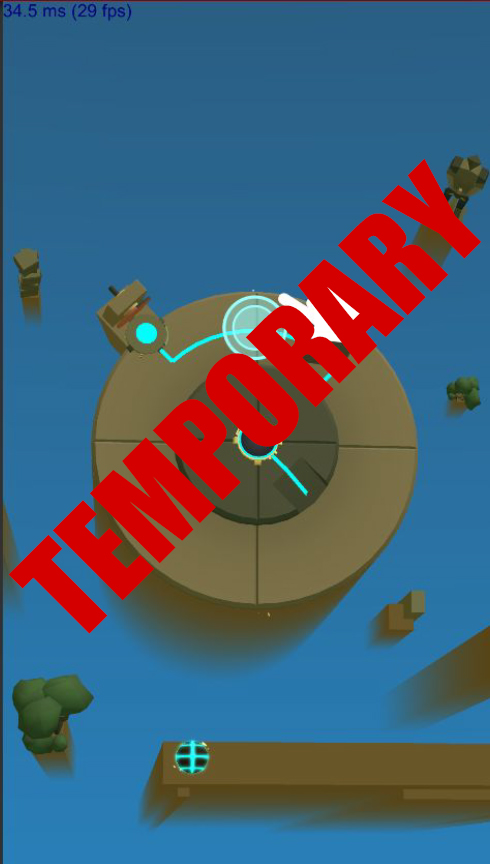
\includegraphics[height=8cm]{fig/tmp.jpg}
	\caption{Wygląd przykładowego poziomu gry \textit{Sphaze}.}
	\label{fig:sphaze_1}
\end{figure}

Osoba grająca nie ma wpływu na ruch sfer, jedynie na obrót pierścieni planszy. Każda rotacja na tych elementach powoduje zmianę połączeń między ścieżkami na nich się znajdującymi. Kule cały czas poruszają się do przodu, chyba że spotkają na swojej drodze skrzyżowanie. Wybierają wtedy ścieżkę, którą zdefiniować można jako "najbardziej prawą". Oznacza to, mając możliwość skręcenia w~prawo, zawsze wybiorą tą opcję. Gdy nie ma możliwości obrotu w~prawo, sprawdzane jest, czy dostępna jest ścieżka na wprost. w~następnej kolejności przeprowadzony zostaje test, czy istnieje skręt w~lewo. w~przypadku braku możliwości wyboru żadnej z przedstawionych opcji, uznawane jest, że natrafiono na "ślepy zaułek", konieczne jest zatem zawrócenie.

Użytkownik decyduje również, z którego miejsca na planszy ma wystartować jaka sfera. Wprowadzenie pierwszej kuli na strefę labiryntu traktowane jest jako rozpoczęcie rozgrywki. Przykładowe punkty startowe, na których ustawić można kule ukazane zostały na rysunku \ref{fig:sphaze_startpoints_1}. Zauważyć można, iż znajdują się one wszystkie na obrzeżach planszy. Jest to reguła, którą gracz jest w~stanie bardzo szybko zauważyć. Dzięki temu na późniejszych poziomach gracze nie próbują ich szukać w~żadnym innym miejscu. Z racji na fakt, iż "rozbijają" one okrągłą sylwetkę planszy wyjątkowo łatwo je dostrzec nawet gdy gra aktualnie ich nie wyróżnia. 
Na każdym poziomie zdefiniowane jest ograniczenie czasowe, którego przekroczenie jednoznacznie wiąże się z koniecznością powtórzenia zadanej planszy. Czasomierz, którego zadaniem jest informowanie użytkownika o tym jak dobrze sobie on radzi, rozpoczyna odliczanie wraz z rozpoczęciem rozgrywki, czyli gdy pierwsza kula zacznie poruszać się w~przestrzeni poziomu. 

\begin{figure}[h!]
	\centering
  	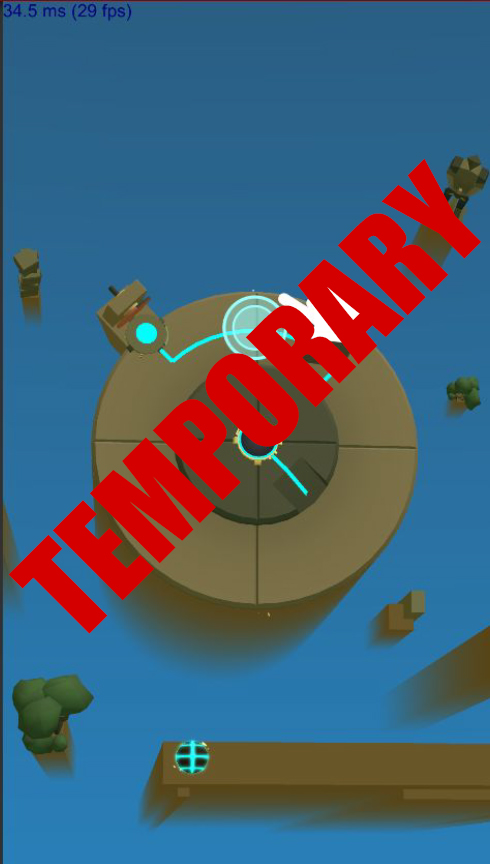
\includegraphics[height=8cm]{fig/tmp.jpg}
	\caption{Przykładowe rozmieszczenie punktów startowych na poziomie. Punkty startowe zostały oznaczone czerwonymi okręgami.}
	\label{fig:sphaze_startpoints_1}
\end{figure}

Gracz ma ograniczoną kontrolę nad rozgrywką, gdyż jego akcje wpływają jedynie pośrednio na jej przebieg. Obrót pierścieni wpływa jednie na możliwości ruchu, jakimi dysponują kule. Zadaniem użytkownika jest dostosowanie się do tego stanu i~przewidzenie, jak obiekty poruszać się będą w~zadanym przez niego środowisku. Nieświadome podejmowanie decyzji może bowiem prowadzić do sytuacji, które szybko potrafią stać się mało zrozumiałe dla użytkownika, który nie do końca rozumie, co się dzieje w~przestrzeni gry.

	\subsection{Samouczki}
Wymagane jest zatem, by gracz przyswoił podstawowe prawa tej gry jak najszybciej. w~przeciwnym wypadku spodziewać się można, iż prędko zacznie odczuwać frustrację spowodowaną pozornie małym wpływem jego akcji na finalny wynik gry. 

Z tego też powodu przygotowane zostały tzw. samouczki mające na celu wyjaśnienie użytkownikowi kluczowych mechanik. Nowe informacje przekazywane są stopniowo. Każdy kolejny element kluczowy jest najpierw przedstawiany w~prostym, kontrolowanym środowisku, a~następnie powtarzany już w~coraz bardziej złożonych sytuacjach. 
W przeprowadzanym badaniu analizowane były trzy główne mechaniki: 
\begin{itemize}
\item sposób na startowanie rozgrywki na danym poziomie, 
\item obracanie pierścieniami,
\item ruch kulek (fakt, iż zawsze skręcają one w~najbardziej prawą ścieżkę.
\end{itemize}

W celu poprawnego nauczenia tych mechanik przygotowane zostały dwa testowe poziomy. w~pierwszym z nich przedstawiane są podstawowe dwie zasady gry. Akcja jaką, użytkownik ma wykonać zostaje przedstawiona wizualnie bez użycia tekstu. Sam gracz musi zrozumieć, że jego ruchem powinno być odzwierciedlenie tego, co pokazywane mu jest na ekranie. Należy zauważyć, że użytkownik nie zawsze jest w~stanie również przewidzieć co się wydarzy, gdy wykona zadane mu zadanie. Dopiero po wykonaniu ukazanej akcji jest w~stanie przeanalizować jaki wpływ miały jego ruchy na przestrzeń gry.
Wygląd poszczególnych etapów tego poziomu dla jednej wersji gry przedstawiony został na rysunku \ref{fig:tut_L1_1}.

\begin{figure}[h!]
	\centering
  	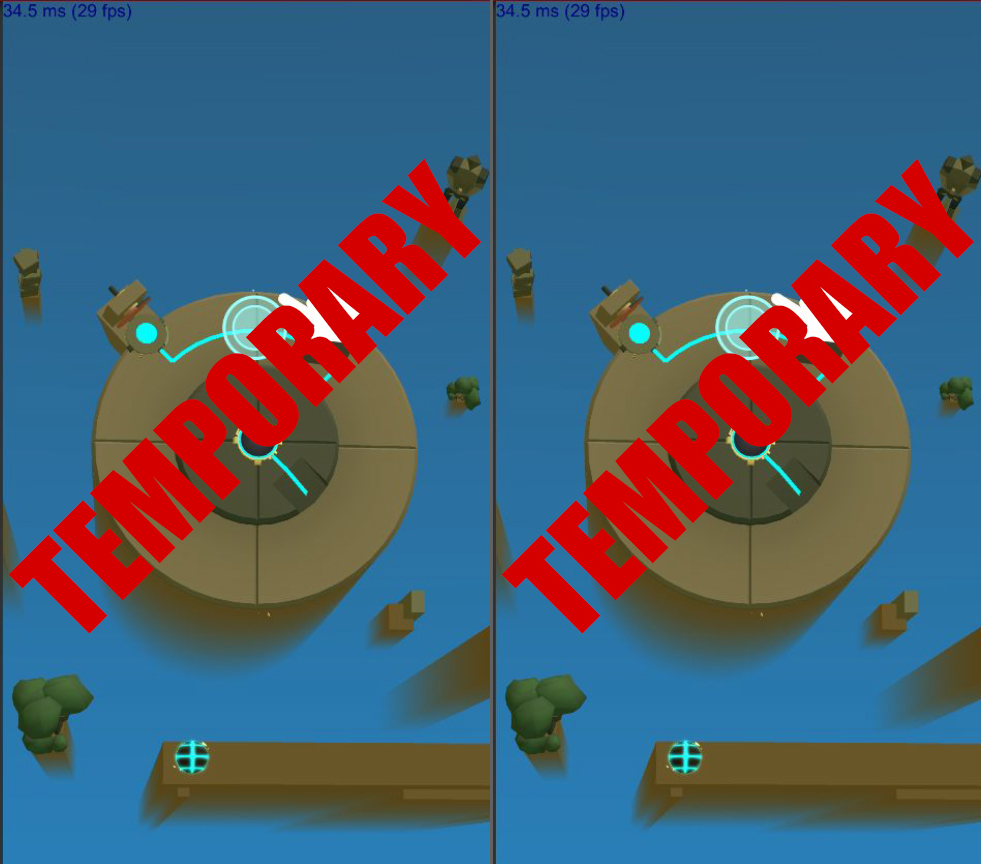
\includegraphics[height=8cm]{fig/tmp2.jpg}
	\caption{Wygląd pierwszego samouczka przed którym postawiony jest gracz.}
	\label{fig:tut_L1_1}
\end{figure}

Plansza dla tego poziomu składa się z dwóch poziomu składa się z dwóch pierścieni. Nie można poruszać pierścieniem w~samym środku, co sprawia, że jedynym fragmentem labiryntu, z którym użytkownik może wchodzić w~interakcję jest zewnętrzny pierścień.
Gdy gracz włączy ten poziom wymagane jest od niego aby najpierw obrócił właśnie ten element. Celem jest doprowadzenie do połączenia ścieżek znajdujących się na pierścieniach. Gdy gracz wykona ruch powodujący rozłączenie tych dróg, samouczek powróci do tego etapu. Pozwala to w~łatwy sposób uzmysłowić użytkownikowi, o wadze, jaką ma stworzenie odpowiedniej drogi dla kul. 
Następnym zadaniem jest ustawienie jedynej sfery na poziomie w~jej miejscu startowym. Samouczek znika dopiero w~momencie poprawnego wykonania tej akcji. Gdy to nastąpi i~użytkownik nie wprowadzi dalszych zmian w~obrocie pierścieni, kula w~szybki sposób dociera do środka labiryntu, a~co za tym idzie - kończy poziom.

Drugi samouczek ustawiony został dopiero na trzeciej planszy. w~tym miejscu chcemy zwrócić uwagę gracza na zachowanie kul w~momencie dotarcia do skrzyżowania. Wygląd tego poziomu zobaczyć można na rysunku \ref{fig:tut_L3_1}. Labirynt w~tym wypadku składa się z trzech pierścieni, z czego z dwoma z nich użytkownik może wejść w~interakcję. Obecny tutaj samouczek wyzwala się dopiero w~momencie, gdy za przeprowadzonymi wcześniej akcjami gracza sfera dotrze do skrzyżowania znajdującego się na środkowym pierścieniu. Zostaje wtedy zabrana użytkownikowi kontrola a~kamera skupia się na problematycznym miejscu. Oprócz tego, zanim zostanie wykonany manewr kulki, zostaje pod nią narysowana strzałka wskazująca, w~którą stronę ona skręci. Gry kulka opuszcza skrzyżowanie, kamera wraca do podstawowej pozycji a~ruchy gracza znowu wpływają na układ pierścieni. Całość opisanych akcji zajmuje podczas normalnej gry tylko ułamek sekundy, dlatego czas gry zostaje w~tym momencie czterokrotnie spowolniony. 
\begin{figure}[h!]
	\centering
  	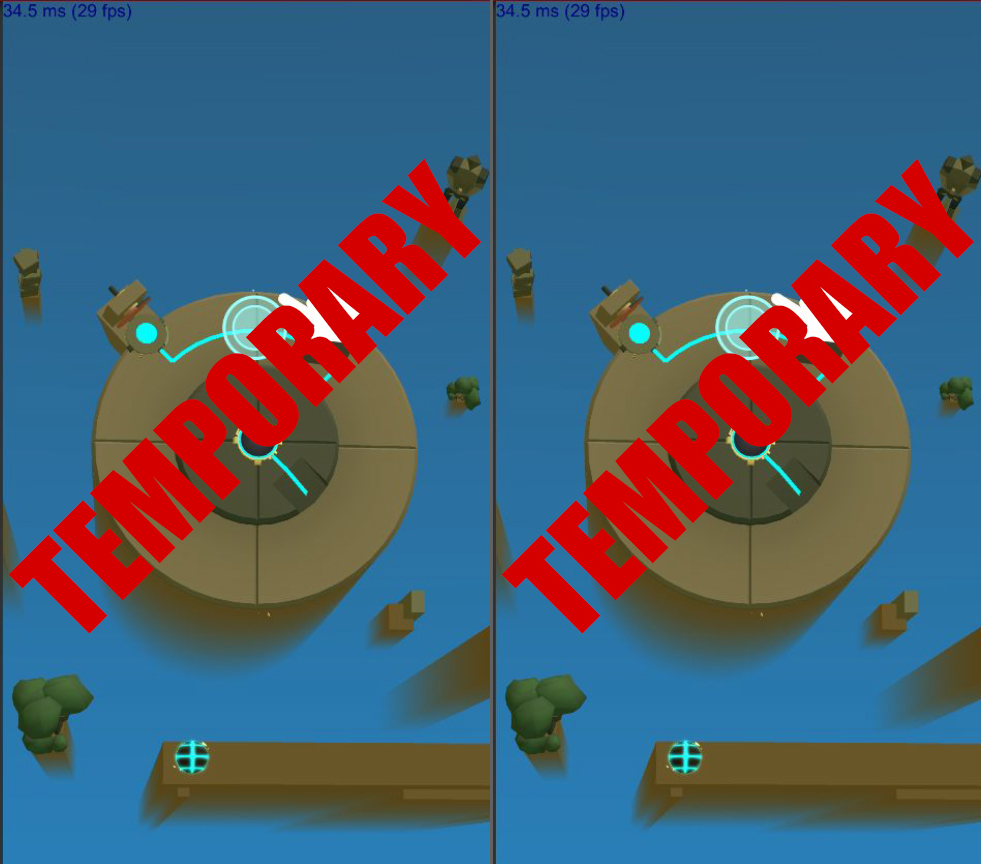
\includegraphics[height=8cm]{fig/tmp2.jpg}
	\caption{Wygląd poziomu zawierającego samouczek tyczący się skrętu kul. Czerwonym okręgiem zaznaczone zostało skrzyżowanie.}
	\label{fig:tut_L3_1}
\end{figure}
Mimo tego, całość przedstawionych operacji trwa niecałe trzy sekundy. Oprócz tego składa się z ruchów kamery, które użytkownik widzi jedyny raz w~tym miejscu rozgrywki. Istnieje zatem szansa, iż nie uda mu się zrozumieć pełnego przekazu, który miał być zawarty w~tym samouczku. Dlatego też następne dwa poziomy, które zobaczyć można na rysunku \ref{fig:tut_L3_2}, stworzone zostały z myślą o tym, by pomóc graczom ze zrozumieniem mechaniki skrętu kul. w~obydwu tych poziomach rozwiązanie, które jest początkowo sugerowane, powoduje powstanie sytuacji, w~której kulka skręcając w~prawo oddala się od środka labiryntu. Użytkownicy, którzy nie rozumieją jeszcze sposobu poruszania się kulki bardzo szybko są wtedy w~stanie zauważyć, że kryje się za tym jakiś algorytm. Gdy to zostanie osiągnięte, zrozumienie w~jaki sposób wyznaczana jest trasa dla sfery przychodzi znacznie łatwiej.

\begin{figure}[h!]
	\centering
  	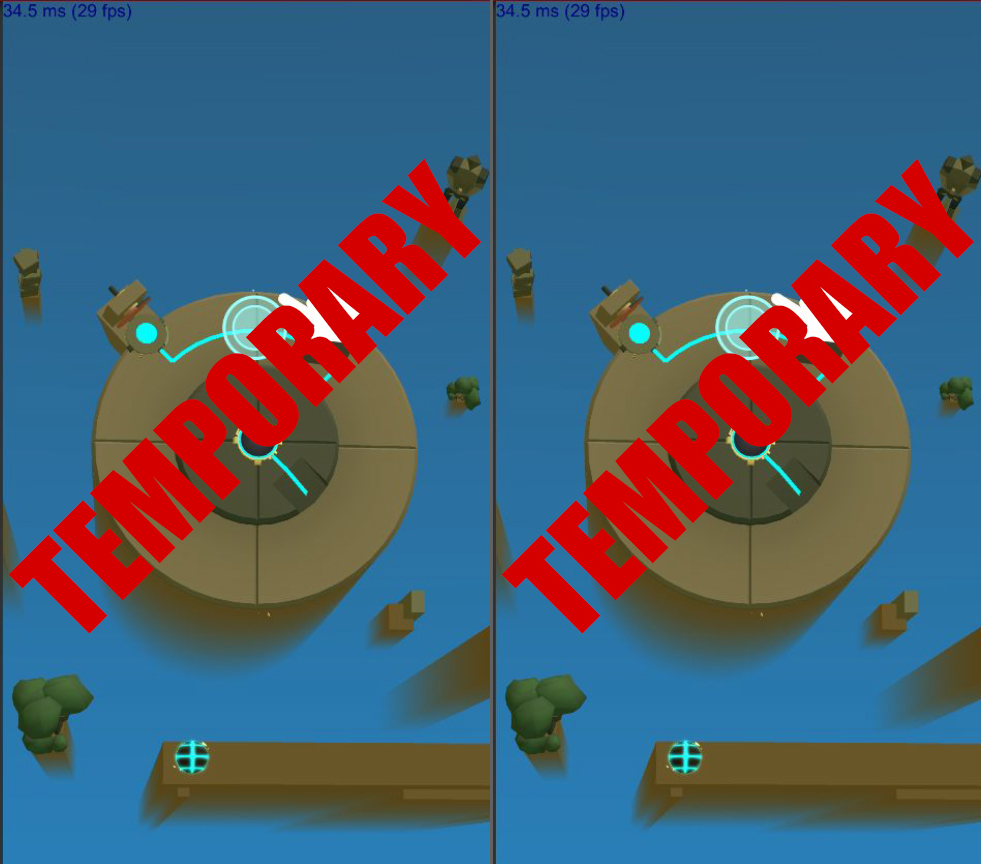
\includegraphics[height=8cm]{fig/tmp2.jpg}
	\caption{Początkowy wygląd czwartego i~piątego poziomu gry \textit{Sphaze}. Mają one na celu pomóc użytkownikowi zrozumieć mechanikę ruchu kul.}
	\label{fig:tut_L3_2}
\end{figure}

\section{Heurystyki}
Z listy heurystyk PLAY \cite{ArticlePLAY} wybrane zostały dwie zaliczające się do kategorii użyteczności oraz mechanik gry. Określają one, jak projektowana powinna być gra, by grywalność była jak największa. Wyróżnione heurystyki zostały wybrane jako nietrywialne i~subiektywnie najprostsze do efektywnego zweryfikowania. Opisane one zostały w~tabeli \ref{tab:tab1}.

\begin{table}[h!]
  \centering
  \caption{Wybrane analizowane heurystyki PLAY z dziedziny informacji o statusie i~wyniku.}
  \label{tab:tab1}
  \begin{tabular}{|r|l|}
    \hline
    1. & Wskaźniki wyniku są płynne, oczywiste, dostępne oraz nie wpływają na rozgrywkę.\\
    \hline
    2. & Sterowanie jest intuicyjne i~mapowane w~sposób naturalny.\\
    \hline
  \end{tabular}
\end{table}

\section{Rodzaje interfejsów}
W rozgrywce widoczny jest jedynie jeden wskaźnik statusu - określa on pozostały użytkownikowi czas na poziomie. Przedstawić go można jako jako dwuwymiarowy przycisk podobny do tego, który używany jest do zatrzymania gry, lub jako siatkę w~przestrzeni gry. Każde podejście ma swoje zalety. w~przypadku elementu 2D użytkownik nie ma wątpliwości co do jego informacyjnego przeznaczenia. Dla wersji w~świecie gry nie zawsze to musi być spełnione. Wręcz przeciwnie, użytkownik, który dopiero uczy się na czym polegają mechaniki gry może odczuć frustrację bądź zniechęcenie wywołane tym, że nie jest możliwe wejście w~interakcję z elementem umieszczonym w~bezpośredniej przestrzeni gry. Plusem tego rozwiązania jest dużo bardziej zrozumiałe połączenie między fragmentami rozgrywki. Prostszym zdaje się zrozumienie powodu startowania czasomierza w~chwili ustawienia pierwszej kulki na planszy, gdy zarówno labirynt, jak i~reprezentacja zegara współdzielą ze sobą jedną przestrzeń.

Spełnianie drugiej z wybranych heurystyk określić można jako sterowanie zbliżone do tego, jak wyglądałoby wykonywanie akcji z gry w~normalnym świecie. Tak więc, aby obrócić pierścień naturalnym zdaje się ruch przeciągania. Również przeniesienie kulki z miejsca na miejsce wydaje się oczywiste, że powinno zostać wykonane poprzez "złapanie" jej i~przeciągnięcie w~miejsce docelowe gdzie finalnie następuje jej "upuszczenie". Dzięki takiemu podejściu do tych mechanik uzyskane zostaje wrażenie fizyczności obiektów w~przestrzeni gry. Stworzona zostaje iluzja, że zachodzi faktyczna interakcja z obiektami, które wyświetlane są na ekranie. Inaczej prezentuje się to przy mniej realnej wersji interakcji. Wykorzystana w~niej zostaje inna znana mechanika z urządzeń mobilnych - proste kliknięcie w~interesujące nas miejsce. Tym sposobem użytkownik jest w~stanie zakomunikować, w~którą stronę chce obrócić pierścień poprzez dotknięcie go z odpowiedniej strony. Przeniesienie kulki w~tym scenariuszu odbywa się poprzez dotknięcie wybranej sfery, a~następnie powtórzenie tej akcji dla miejsca docelowego. w~tym wypadku użytkownik, który dobrze rozumie te mechaniki może znacznie szybciej wykonywać akcje w~trakcie gry. Wiąże się to jednak z utratą części wiarygodności, którą uzyskać można było sposobem pierwszym.

Na podstawie wybranych heurystyk przygotowane zostały zatem cztery wersje gry. Każda z nich spełnia inną kombinację zadanych założeń. Takie podejście pozwala na dokładne przetestowanie, jaki wpływ zasady te mają na grywalność aplikacji. 
\subsection{Interfejs Swipe 2D}
Jako pierwszy wyróżniony został interfejs \textit{Swipe 2D}, który w~założeniu spełnia zarówno pierwszą, jak i~drugą heurystykę. Jego reprezentację graficzną dla pierwszego poziomu gry zobaczyć można na rysunku \ref{fig:interface_Swipe_2d}. Zegar zdefiniowany jest w~nim jako element dwuwymiarowy znajdujący się w~górnej części ekranu, a~wszelkie interakcje rozwiązane są poprzez jak najwierniejsze odwzorowanie ich odpowiedników z rzeczywistości. Spodziewać się zatem można najmniejszej ilości błędów popełnianych przez użytkowników już od samego początku gry. Również różnice w~czasach pojedynczego testu powinny być dla tej wersji względnie niewielkie.
\begin{figure}[h!]
	\centering
  	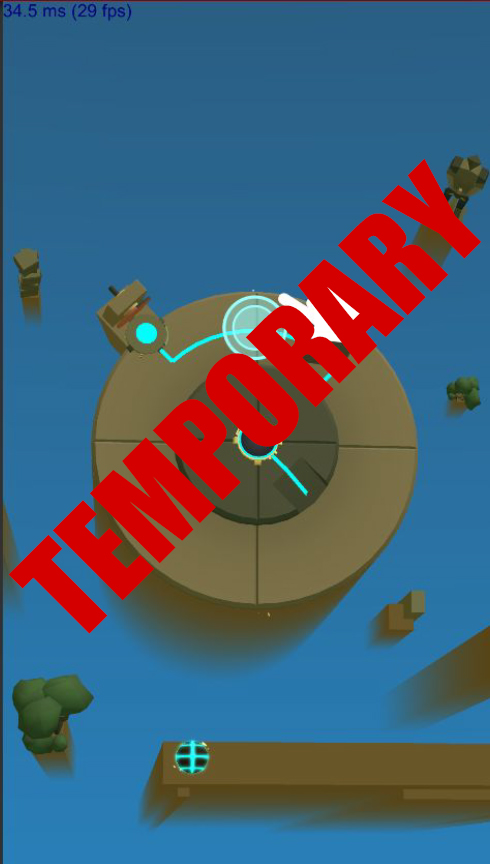
\includegraphics[height=8cm]{fig/tmp.jpg}
	\caption{Wygląd poziomu pierwszego dla wersji gry wykorzystującej interfejs \textit{Swipe 2D}.}
	\label{fig:interface_Swipe_2d}
\end{figure}
\subsection{Interfejs Swipe 3D}
Wersja interfejsu wykorzystująca mechanikę przesuwania lecz niespełniająca pierwszej z wybranych heurystyk określona została mianem \textit{Swipe 3D}. Jego wygląd zaprezentowany jest na rysunku \ref{fig:interface_Swipe_3d}. Siatka stanowiąca zegar umieszczona została w~świecie gry, jako element znajdujący się wizualnie przy wyborze kul. Położenie to zostało zmienione z racji na charakterystyczne ustawienie kamery w~grze. Nie pozwala ono na ustawienie tak ciężkiego elementu powyżej labiryntu, gdyż wpływałoby to negatywnie na estetykę gry. To rozwiązanie wpływać może rozgrywkę, gdyż niewykluczona jest sytuacja, w~której gracz może odbierać czasomierz jako element, z którym  należy wejść w~jakąś interakcję. Spodziewać się tu można zatem większej ilości błędów, które popełniane mogą być przy pierwszej styczności użytkownika z grą.
\begin{figure}[h!]
	\centering
  	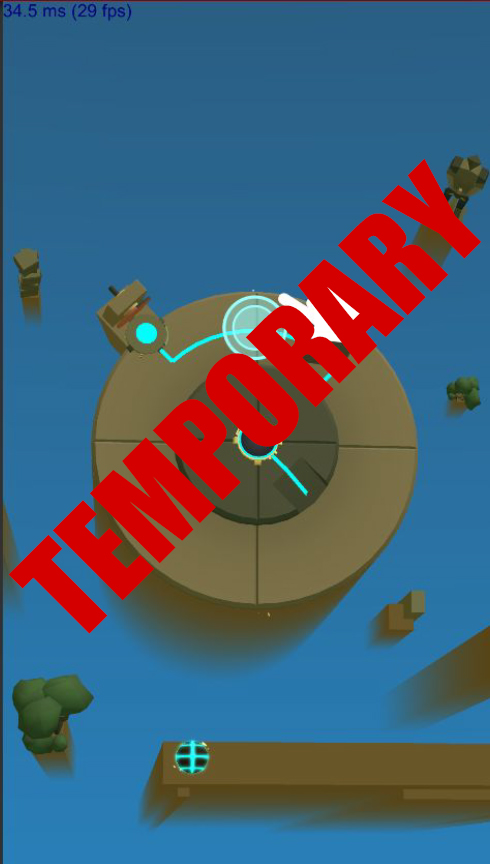
\includegraphics[height=8cm]{fig/tmp.jpg}
	\caption{Wygląd poziomu pierwszego dla wersji gry wykorzystującej interfejs \textit{Swipe 3D}.}
	\label{fig:interface_Swipe_3d}
\end{figure}
\subsection{Interfejs Click 2D}
Interfejs \textit{Click 2D} wizualnie nie rózni się od wersji \textit{Swipe 2D}. Zmieniony jest tu jednak styl sterowania głównymi mechanikami gry na takie, które są w~znacznie mniejszym stopniu reprezentacją rzeczywistych interakcji. Cechują się one tym, że by osiągnąć ten sam cel wykonywane mogą być znacznie szybsze ruchy (kliknięcie zamiast przesuwania palca po ekranie). Oznaczać to może, że doświadczony użytkownik jest w~stanie uzyskać w~tej wersji lepsze czasy niż ten, który umiejętnie posługuje się wersją z mechaniką przesuwania. Idąc tym tropem założyć można, iż różnica w~czasach przechodzenia poszczególnych poziomów będzie zatem tutaj zauważalnie większa, gdyż wymaga on nauczenia się mniej intuicyjnej zasady gry.
\subsection{Interfejs Click 3D}
Podobnie jak w~poprzednim przypadku, w~wersji interfejsu \textit{Click 2D} brak jest różnic wizualnych względem \textit{Swipe 2D}. w~tym wypadku jednak nie jest spełniona żadna ze sprawdzanych heurystyk. Oznaczać to może, że wyniki dla tego wypadku będą najmniej korzystne. Spodziewać się można dużej ilości początkowych błędów spowodowanych mniej odciętym od całości gry zegarem oraz większych różnic w~statystykach podczas przechodzenia tego samego poziomu dwukrotnie przez pojedynczego gracza.
\section{Struktura badania}
Na potrzeby przeprowadzenia testów przygotowane zostało badanie mające na celu wydobycie z przebiegów gry przydatnych informacji. 
Użytkownik miał za zadanie zagrać w~przygotowaną wcześniej grę w~ściśle określony sposób:
\begin{itemize}
\item przejść pierwszych pięć poziomów,
\item zagrać w~arbitralnie dobraną liczbę następnych plansz (przynajmniej 5),
\item ponownie rozegrać pierwszych pięć poziomów.
\end{itemize}

Zestawienie początkowych ustawień wszystkich pięciu poziomów zawarte zostało na rysunku 
\begin{figure}[h!]
	\centering
  	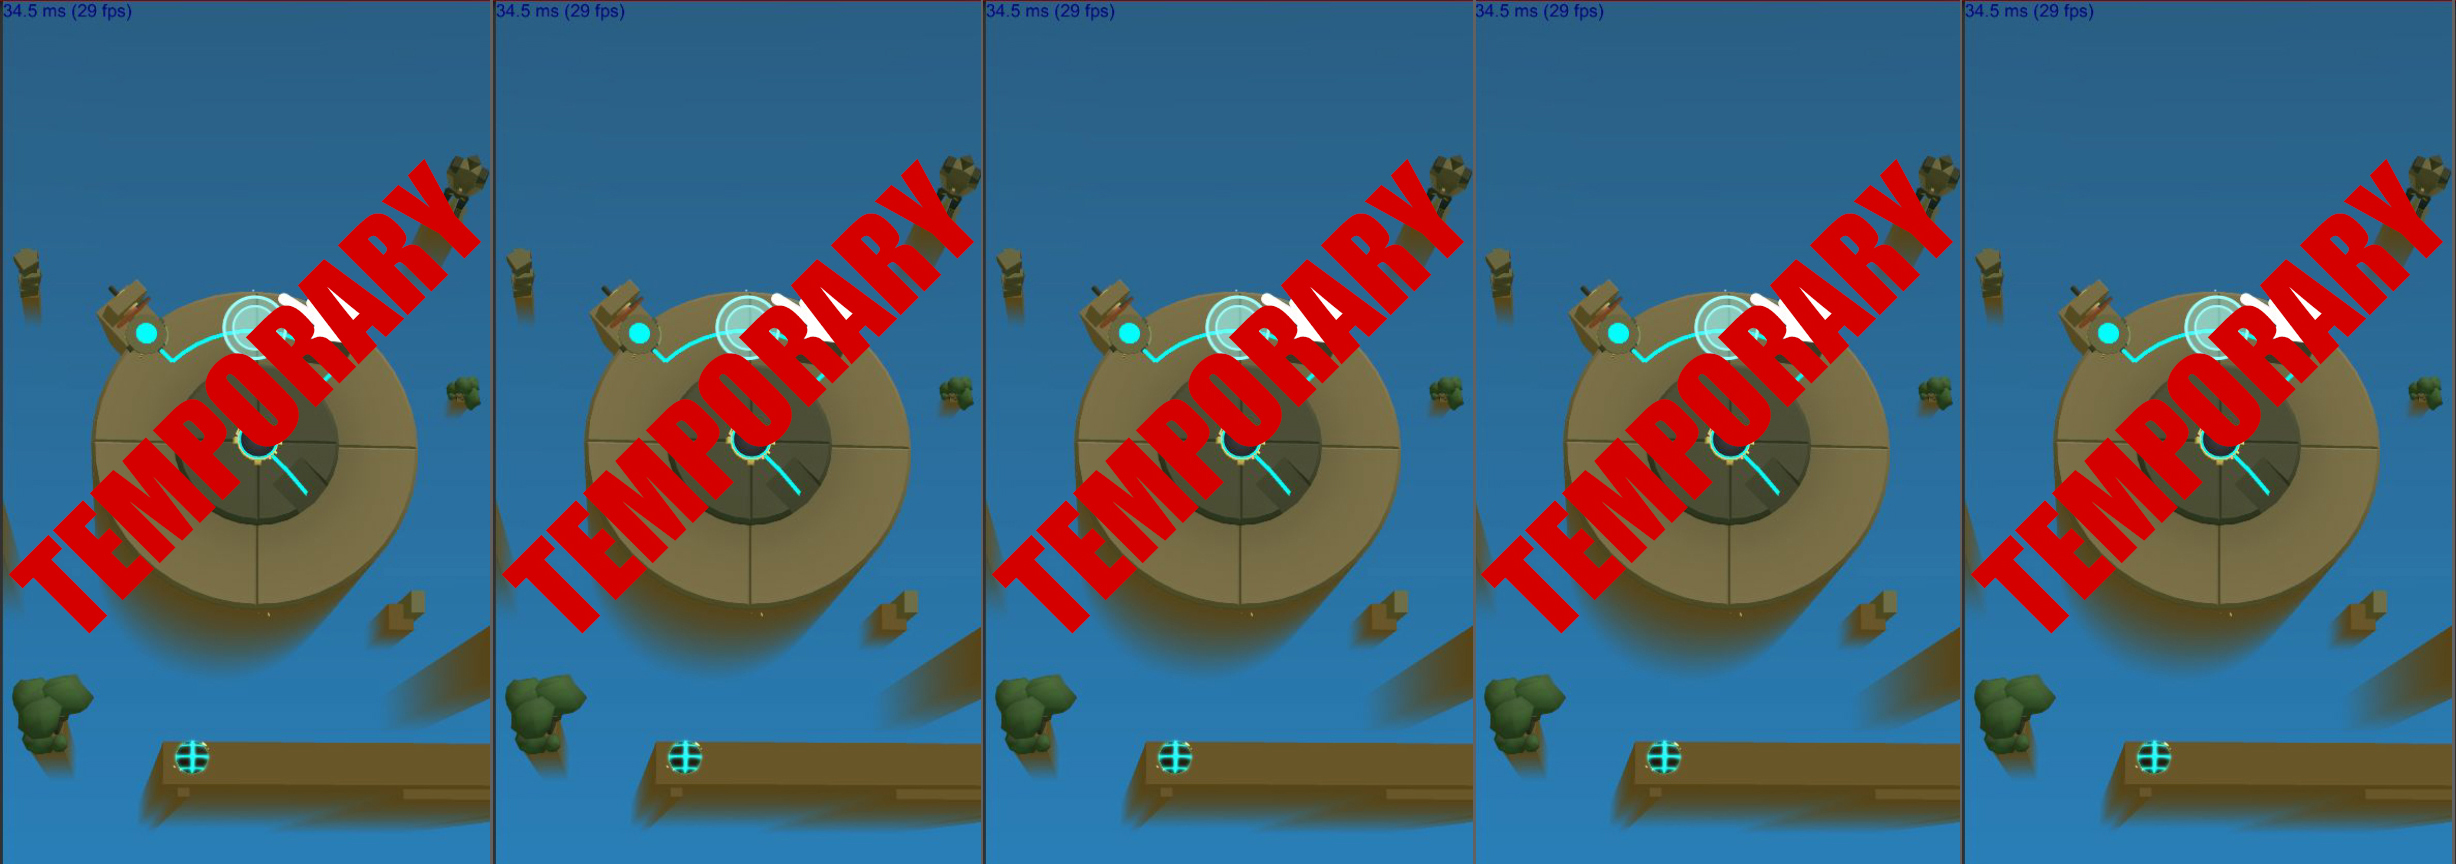
\includegraphics[width=\linewidth]{fig/tmp5.jpg}
	\caption{Wygląd początkowy pierwszych pięciu poziomów gry \textit{Sphaze}. Poziomy ustawione są w~kolejności, od poziomu pierwszego (po lewej) do piątego (po prawej).}
	\label{fig:all_levels}
\end{figure}
Zarówno przed jak i~po przeprowadzeniu badania osoba testująca nie musiała wypełniać żadnej ankiety odnośnie swoich wrażeń z gry. Oznacza to też, iż dane takie jak płeć, czy wiek gracza nie były brane pod uwagę w~dalszej ocenie wyników. Gra automatycznie zapisywała wyniki badania do pliku, który później podlegał analizie.

Zauważyć należy iż dane zbierane były tylko dla pierwszych pięciu plansz. Powtórzenie ich przejścia na koniec indywidualnego testu jest kluczowe dla wyników badań. Przy pierwszym podejściu do poziomów 1-5 gracz nie wie, czego aplikacja może od niego wymagać. Jest to jego pierwsze starcie z mechanikami, których musi się nauczyć. \
Inaczej sprawa się ma z drugimi wynikami danej osoby badanej. Z racji tego, że wymagane jest by przeszła ona przynajmniej 10 poziomów, założyć można, iż zaznajomiła się ona z podstawowymi prawami gry. Różnice pomiędzy tymi wynikami pozwalają na określenie jak dużego postępu dokonał gracz, o ile lepiej zrozumiał zadane mechaniki. Zminimalizowana zostaje w~ten sposób różnica pomiędzy umiejętnościami różnych osób. Gdy porównywane są one do samych siebie nie nie trzeba brać pod uwagę czynników, takich jak przykładowo predyspozycje do sprawnego przechodzenia gier logicznych.

Pomijalny staje się również wpływ, jaki miało środowisko, w~którym przeprowadzany był eksperyment. w~uproszczeniu założyć można, że w~warunkach, jakie były zapewnione użytkownikom zarówno oświetlenie, jak i~poziom hałasu utrzymywał się na jednym poziomie dla jednego testu.

Same testy odbywały się zarówno na wyciszonym, względnie odizolowanym pomieszczeniu ale także w~dużo trudniejszych warunkach - jako część większych wydarzeń, bądź podczas jazdy komunikacją miejską. 

Do celów badania przygotowane zostały cztery wersje gry, które zawierały w~sobie opisane wcześniej interfejsy. Osobie badanej przyznawana była losowo wybrana aplikacja z tej puli i~przedstawiana była jako jedyna wersja gry. 
Badane były osoby, które nigdy wcześniej nie spotkały się z grą będącą obiektem testów. Miały one za zadanie przejść zadane poziomy bez żadnej wcześniejszej informacji o tym, jaki jest chociażby warunek przejścia do następnej planszy. Informacja o tym, że wyniki podlegają zapisowi przekazywana była dopiero wtedy, gdy wymagane było, by osoba testowana przystąpiła ponownie do pierwszych pięciu poziomów. Miało to na celu możliwe zminimalizowanie presji czasu, która mogłaby się pojawić przy otrzymaniu aplikacji do testowania.(JAKIŚ LINK?)

Dla każdego przejścia poziomu przez danego użytkownika zebrane zostały następujące dane:
\begin{itemize}
\item czas absolutny, 
\item czas ruchu kuli,
\item ilość obrotów pierścieni,
\item ilość dotknięć ekranu.
\end{itemize}
Oprócz tego, obliczona została dodatkowa zmienna, która zależna jest od czasu absolutnego oraz czasu ruchu kuli - czas myślenia użytkownika.

	\subsection{Czas absolutny}
Czas, który użytkownik potrzebował na przejście poziomu, licząc od jego załadowania określany jest mianem absolutnego $t_{abs}$. Zawiera on w~sobie długość trwania obejrzanej przez użytkownika animacji wejścia poziomu, a~jego liczenie przerywane jest wraz z wejściem ostatniej kuli na poziomie do środka labiryntu. Czas ten nie zawiera zatem w~sobie informacji o tym, jak długo użytkownik pozostawał na ekranie podsumowującym dany poziom. Spowodowane to było obserwacją, że czas spędzony w~tym ekranie uznany został za pomijalny w~przeprowadzanych badaniach.
	\subsection{Czas kuli}
Oprócz obliczania tego, ile czasu potrzebne było użytkownikowi na przejście poziomu wymiernym okazało się również sprawdzanie jak optymalne ścieżki wybrane zostały dla sfer. Wszystkie plansze, które wykorzystane zostały w~badaniu korzystały tylko z jednej kulki, która na każdej z nich poruszała się z tą samą szybkością. Oznacza to, że droga ta jest wprost proporcjonalna do czasu, w~jakim poruszała się kulka - $t_{ball}$. Jego obliczanie zaczyna się wraz z wykonaniem przez użytkownika akcji startu sfery w~wybranym punkcie startowym labiryntu, a~kończy się, podobnie jak w~przypadku $t_{abs}$, wraz z dotarciem tej sfery do środka. Im większa ta zmienna, tym bardziej można przypuszczać, iż użytkownik nie przewidział, jak zachowa się kula na planszy. Zaobserwować można tutaj, w~zależności od urządzenia na którym przeprowadzone zostały pomiary, iż zmienna ta jest obciążona błędem pomiaru rzędu $5 ms$.
	\subsection{Czas myślenia}
Przydatnym w~celach analizy wyników okazał się również czas myślenia - $t_{think}$. Opisać go można zależnością $t_{think} = t_{abs} - t_{ball}$. Określa on, jak długo zajęło użytkownikowi opracowanie, w~jaki sposób powinien podejść do przejścia poziomu. Wyekstrahowanie go z pozostałych dwóch czasów pozwoliło w~prosty sposób porównywać stosunek czasu poświęconego na planowanie do tego, jaki zajęło wprowadzanie tego planu w~życie przez danego użytkownika.
	\subsection{Ilość obrotów}
Jednym z kluczowych aspektów gry testowej są pierścienie, z których składają się labirynty na poziomach. Można je obracać zarówno przed rozpoczęciem ruchu kulek, jak i~w jego trakcie. Dla każdego poziomu zdefiniowana jest minimalna ilość obrotów konieczna do jego przejścia ($r_{rotMin}$). w~trakcie rozgrywki zliczana jest ich ilość, jakie wykonał użytkownik i~oznaczana jako $r_{rot}$. 

Częsta sytuacja, gdy $r_{rot} > r_{rotMin}$  może zatem być wyznacznikiem tego, iż użytkownik nie przewidział jakiejś sytuacji, która pojawiła się w~rozgrywce i~musiał improwizować podczas, gdy czasomierz odmierzał już ilość sekund pozostałych do końca poziomu. Innym wyjaśnieniem znacznej ilości obrotów pierścieni na poziomie może również być fakt, iż gracz mógł zechcieć przed rozpoczęciem faktycznej rozgrywki wizualnie zobaczyć interesujące go kombinacje obrotów i~opracować plan działania. Rozróżnić można, z którą sytuacją mamy do czynienia poprzez porównanie relacji czasów $t_{think}$ oraz $t_{ball}$ do tych wyznaczonych poprzez ich odpowiedniki referencyjne - $t_{thinkMin}$ i~$t_{ballMin}$.
	\subsection{Ilość dotknięć ekranu}
Zliczane również jest każde dotknięcie ekranu, jakie wykonał użytkownik podczas rozgrywki (oznaczane jako $c_{scr}$). Po ich stosunku względem ilości obrotów pierścieni wywnioskować można, jak dobrze użytkownik rozumiał, jakie operacje musi wykonać, by przejść poziom. Gdy $\frac{c_{scr}}{r_{rot}} >> 1$ oznacza to, że mechaniki obrotu pierścieni i~startowania kulki nie są dla użytkownika intuicyjne, popełnia przy nich błędy. Innym wytłumaczeniem może być również niezrozumienie szaty graficznej aplikacji, a~co za tym idzie zgadywanie, z którymi elementami gry można wchodzić w~interakcję. Liczbę wszystkich błędów dotknięć, jakie użytkownik popełnił w~trakcie przechodzenia danego poziomu obliczyć można z następującego wzoru:
\begin{equation}
\label{eq_errors}
c_{err} = c_{scr} - r_{rot} - c_{start},
\end{equation}
gdzie  $c_{start}$ oznacza liczbę kliknięć potrzebnych do wystartowania jednej kulki w~danej wersji gry. Dla interfejsów wykorzystujących mechanikę \textit{Swipe} jest to $c_{start} = 1$, podczas gdy dla interfejsów typu \textit{Click} wynosi ono $c_{start} = 2$.
\section{Analiza danych}
Zebrane dane rozdzielone zostały ze względu na wersje gry, dla której były zarejestrowane. W ramach i-tego parametru zdefiniowany został został zbiór $X = \{x_{i,1},x_{i,1},..., x_{i,n}\}$. gdzie n oznacza ilość zebranych danych dla danej wersji interfejsu. W celu wyeliminowanie wątpliwości związanych z wielkościami prób czy innymi czynnikami, które wpłynąć by mogły na czytelną analizę zebranych informacji przetworzono je za pomocą wybranych miar tendencji centralnej, rozproszenia oraz kształtu rozkładu \cite{online_Statistics}.

\subsection{Miary tendencji centralnej}
Miary tendencji centralnej wykorzystywane są w celu wyznaczenia największej koncentracji wyników. Do analizy wyników, które zostały zebrane w trakcie badań wykorzystane zostały średnia arytmetyczna oraz mediana.
\begin{itemize}
\item
Średnia arytmetyczna (ang. \textit{mean}) - oznacza wartość, w której znaleźć można największe skupiska pomiarów. 
Wyliczona była ona z następującego wzoru:
\begin{equation}
\label{eq_mean}
\overline{x} = \frac{1}{n}\sum_{i=1}^{n}x_{i},
\end{equation}
gdzie $x_{i}$ to wartość i-tego pomiaru.
%Miara tendencji centralnej, wartość, wokół której grupują się pomiary. 

\item
Kwartyle (eng. \textit{quartile}) - wartości zmiennej, które oddzielają informacje w zbiorze danych na stosunki, które wynoszą odpowiednio $\frac{l}{4}$. Zmienna $l$ oznacza numer kwartyla i jej wartości zawierają się w zbiorze  $\{1,2,3\}$.

\begin{equation}
\label{eq_quart}
Q_{\frac{l}{4}}=(k+1-(n+1_\frac{l}{4})x_{(k)}+((n+1)\frac{l}{4}-k)x_{k+1},
\end{equation}
gdzie $k = [(n+1)\frac{l}{4}]$ oraz $[a]$ oznacza całkowitą część liczby $a$.

Drugi kwartyl jest stosowany najczęściej i opisywany jest mianem mediany. Dzieli ona zbiór danych na dwie równe części, wyznacza wartość środkową. W celu jej obliczenia można zastosować następujący wzór:
\begin{equation}
\label{eq_median}
Me=\left\{
        \begin{array}{ll}
             x_{(\frac{n+1}{2})}, & n - nieparzyste\\
             \frac{1}{2}(x_{(\frac{n}{2})}+x_{(\frac{n}{2}+1)}), & n - parzyste\\
             \end{array}
        \right.
\end{equation}
%Wartości zmiennej, które dzielą dane na części pozostające ze sobą w odowiednim stosunku. Najczęściej używane kwantyle to kwartyle (podział na 4 części), decyle (podział na 10 części) i percentyle (podział na 100 części). Np. pierwszy kwartyl dzieli dane na dwie części w ten sposób, ze 1/4 z nich ma wartości od niego większe, a 3/4 - mniejsze. 
\end{itemize}

Zauważyć należy, iż w procesie przetwarzania danych pod względem tendencji centralnej pominięta została dominanta. Spowodowane zostało to tym, że zebrane dane to w większości liczby zmiennoprzecinkowe, które mają bardzo małą szansę na powtórzenie się pomiędzy wynikami dwóch różnych osób. Dominanta nie niosła by zatem ze sobą żadnej przydatnej informacji, gdyż określa ona wartość najczęściej występującą.

\subsection{Miary rozproszenia}
Miary rozproszenia definiują wielkość zróżnicowania wyników zawartych w zbiorze danych. Innymi słowy, określają one rozkład zmiennych wokół centralnej wartości. W przeprowadzonej analizie obliczano wartość minimalną i maksymalną, rozstęp, wariancję, odchylenie standardowe a także współczynnik zmienności.
\begin{itemize}
\item
Rozstęp (ang. \textit{range}) - jest to różnica między największą, a najmniejszą wartością w zbiorze danych. Duże jego wartości oznaczają, iż w wynikach zawarte są informacje, które są od siebie bardzo odległe. Nie uwzględnia on jednak tego, jak bardzo dane te są skupione. Obliczany jest ze wzoru:
\begin{equation}
\label{eq_range}
R = x_{max} - x_{min},
\end{equation}
gdzie $x_{max}$ i $x_{min}$ oznaczają odpowiednio wartość maksymalną oraz minimalną zbioru danych.

\item
Wariancja (eng. \textit{variance}) - mierzy jak bardzo dane rozproszone są względem ich średniej wartości. Opisywana jest wzorem:
\begin{equation}
\label{eq_variance}
Var(X) = \frac{1}{n-1}\sum_{i=1}^{n}{(x_{i}-\overline{x})}^2.
\end{equation}
\item
Odchylenie standardowe (eng. \textit{standard deviation}) - pierwiastek z wariancji, mierzy przeciętne odchylenie wyników od ich średniej. Opisać można je poprzez wzór:
\begin{equation}
\label{eq_stddev}
s = \sqrt{Var(X)}.
\end{equation}

\item
Współczynnik zmienności (ang. \textit{coefficient of variation}) - służy do pokazania zakresu różnorodności danych w relacji do ich wartości średniej. Zwykle przedstawiany jest jako wartość procentowa. Opisać można go następującym równaniem:
\begin{equation}
\label{eq_stddev}
V = \frac{s}{\overline{x}}\cdot 100\%.
\end{equation}

Gdy $V$ jest mniejsze bądź równe od 50\% dane określane są jako mało zmienne. Wartość tego współczynnika znajdująca się w zakresie $50\% < V \leq 100\%$ oznacza umiarkowaną zmienność w zbiorze. W sytuacjach, gdy $V > 100\%$ to dane oznaczane są jako bardzo chwiejne.

\end{itemize}

\subsection{Miary kształtu rozkładu}
Miary kształtu rozkładu pozwalają na określenie w jakim stopniu otrzymane dane zbliżone są do rozkładu normalnego. Na potrzeby opracowania zebranych informacji wykorzystano skośność oraz kurtozę.

\begin{itemize}
\item
Skośność (ang. \textit{skewness}) - wyznacza w którą stronę "przechylony" jest opracowywany rozkład zmiennych. Dla dodatnich wartości tego współczynnika większa ilość danych zorientowana jest po "prawej" stronie średniej, dla ujemnego zależność ta jest odwrotna. Przedstawiając rozkład w reprezentacji graficznej dłuższy ogon znajduje się po prawej stronie dla ujemnych skośności, po lewej dla dodatnich.
\begin{equation}
\label{eq_skew}
Sk = \frac{n\sum_{i=1}^{n}(x_i-\overline{x})^3}{(n-1)(n-2)s^3}
\end{equation}

\item
Kurtoza (ang. \textit{kurtosis}) - mierzy jak duże skupienie jest danych wokół średniej. Większe jej wartości definiują mocniejsze koncentracje dla wartości centralnej. Jej znak określa relacje danych względem rozkładu normalnego. Jeżeli kurtoza jest dodatnia, to opracowywany zbiór zdefiniowany jest rozkładem bardziej od niego smukłym, zaś ujemne jej wartości definiują dane bardziej 'płaskie'. Opisuje się ją wzorem:
\begin{equation}
\label{eq_kurtosis}
K = \frac{n(n+1)\sum_{i=1}^{n}(x_i-\overline{x})^4-3(n-1)(\sum_{i=1}^{n}(x_i-\overline{x})^2)^2}{(n-1)(n-2)(n-3)s^4}.
\end{equation}
\end{itemize}

\section{Wyniki referencyjne}
Przydatnymi do oceny tego, jak dobrze gracze są w~stanie poradzić sobie na określonych poziomach w~danej wersji gry są dane referencyjne. Określają one zapewnione przez twórców najlepsze wyniki, jakie można uzyskać dla mierzonych parametrów bez przyśpieszania domyślnych animacji gry. Zauważyć należy, że przy pomiarach tych informacji jedyny istotny podział między wersjami gry to to, czy interfejs wykorzystuje interakcje za pomocą kliknięć czy przesunięć. Wartości te zamieszczone zostały w~tabeli \ref{tab:ref_data}.

\begin{table}[H]
  \centering
  
  \caption{Dane referencyjne gry \textit{Sphaze} dla interfejsów Click oraz Swipe.}
  %\resizebox{\textwidth}{!}{%
	
    \begin{tabular}{|c|l|ll|}
    \hline
    \rowcolor[rgb]{ .651,  .651,  .651} \multicolumn{1}{|l|}{lvl} & param & \multicolumn{1}{c}{Swipe} & \multicolumn{1}{c|}{Click} \bigstrut\\
    \hline
    \rowcolor[rgb]{ .851,  .851,  .851} 1     & t\_Abs & \cellcolor[rgb]{ 1,  1,  1}10,76 & \cellcolor[rgb]{ 1,  1,  1}11,65 \bigstrut[t]\\
    \rowcolor[rgb]{ .851,  .851,  .851}       & t\_Ball & \cellcolor[rgb]{ 1,  1,  1}2,74 & \cellcolor[rgb]{ 1,  1,  1}2,76 \\
    \rowcolor[rgb]{ .851,  .851,  .851}       & t\_Think & \cellcolor[rgb]{ 1,  1,  1}8,02 & \cellcolor[rgb]{ 1,  1,  1}8,89 \\
    \rowcolor[rgb]{ .851,  .851,  .851}       & rots  & \cellcolor[rgb]{ 1,  1,  1}1 & \cellcolor[rgb]{ 1,  1,  1}1 \\
    \rowcolor[rgb]{ .851,  .851,  .851}       & clicks & \cellcolor[rgb]{ 1,  1,  1}3 & \cellcolor[rgb]{ 1,  1,  1}4 \bigstrut[b]\\
    \hline
    \rowcolor[rgb]{ .851,  .851,  .851} 2     & t\_Abs & \cellcolor[rgb]{ 1,  1,  1}16,15 & \cellcolor[rgb]{ 1,  1,  1}17,40 \bigstrut[t]\\
    \rowcolor[rgb]{ .851,  .851,  .851}       & t\_Ball & \cellcolor[rgb]{ 1,  1,  1}5,97 & \cellcolor[rgb]{ 1,  1,  1}5,99 \\
    \rowcolor[rgb]{ .851,  .851,  .851}       & t\_Think & \cellcolor[rgb]{ 1,  1,  1}10,18 & \cellcolor[rgb]{ 1,  1,  1}11,41 \\
    \rowcolor[rgb]{ .851,  .851,  .851}       & rots  & \cellcolor[rgb]{ 1,  1,  1}2 & \cellcolor[rgb]{ 1,  1,  1}3 \\
    \rowcolor[rgb]{ .851,  .851,  .851}       & clicks & \cellcolor[rgb]{ 1,  1,  1}3 & \cellcolor[rgb]{ 1,  1,  1}5 \bigstrut[b]\\
    \hline
    \rowcolor[rgb]{ .851,  .851,  .851} 3     & t\_Abs & \cellcolor[rgb]{ 1,  1,  1}20,03 & \cellcolor[rgb]{ 1,  1,  1}21,24 \bigstrut[t]\\
    \rowcolor[rgb]{ .851,  .851,  .851}       & t\_Ball & \cellcolor[rgb]{ 1,  1,  1}11,05 & \cellcolor[rgb]{ 1,  1,  1}10,99 \\
    \rowcolor[rgb]{ .851,  .851,  .851}       & t\_Think & \cellcolor[rgb]{ 1,  1,  1}8,98 & \cellcolor[rgb]{ 1,  1,  1}10,25 \\
    \rowcolor[rgb]{ .851,  .851,  .851}       & rots  & \cellcolor[rgb]{ 1,  1,  1}1 & \cellcolor[rgb]{ 1,  1,  1}1 \\
    \rowcolor[rgb]{ .851,  .851,  .851}       & clicks & \cellcolor[rgb]{ 1,  1,  1}3 & \cellcolor[rgb]{ 1,  1,  1}4 \bigstrut[b]\\
    \hline
    \rowcolor[rgb]{ .851,  .851,  .851} 4     & t\_Abs & \cellcolor[rgb]{ 1,  1,  1}12,23 & \cellcolor[rgb]{ 1,  1,  1}15,31 \bigstrut[t]\\
    \rowcolor[rgb]{ .851,  .851,  .851}       & t\_Ball & \cellcolor[rgb]{ 1,  1,  1}3,74 & \cellcolor[rgb]{ 1,  1,  1}3,77 \\
    \rowcolor[rgb]{ .851,  .851,  .851}       & t\_Think & \cellcolor[rgb]{ 1,  1,  1}8,49 & \cellcolor[rgb]{ 1,  1,  1}11,54 \\
    \rowcolor[rgb]{ .851,  .851,  .851}       & rots  & \cellcolor[rgb]{ 1,  1,  1}1 & \cellcolor[rgb]{ 1,  1,  1}1 \\
    \rowcolor[rgb]{ .851,  .851,  .851}       & clicks & \cellcolor[rgb]{ 1,  1,  1}3 & \cellcolor[rgb]{ 1,  1,  1}4 \bigstrut[b]\\
    \hline
    \rowcolor[rgb]{ .851,  .851,  .851} 5     & t\_Abs & \cellcolor[rgb]{ 1,  1,  1}15,22 & \cellcolor[rgb]{ 1,  1,  1}18,26 \bigstrut[t]\\
    \rowcolor[rgb]{ .851,  .851,  .851}       & t\_Ball & \cellcolor[rgb]{ 1,  1,  1}7,01 & \cellcolor[rgb]{ 1,  1,  1}7,01 \\
    \rowcolor[rgb]{ .851,  .851,  .851}       & t\_Think & \cellcolor[rgb]{ 1,  1,  1}8,21 & \cellcolor[rgb]{ 1,  1,  1}11,25 \\
    \rowcolor[rgb]{ .851,  .851,  .851}       & rots  & \cellcolor[rgb]{ 1,  1,  1}1 & \cellcolor[rgb]{ 1,  1,  1}2 \\
    \rowcolor[rgb]{ .851,  .851,  .851}       & clicks & \cellcolor[rgb]{ 1,  1,  1}3 & \cellcolor[rgb]{ 1,  1,  1}5 \bigstrut[b]\\
    \hline
    \end{tabular}%


  %}
  \label{tab:ref_data}%
\end{table}%

\section{Podwójna analiza}
Struktura przeprowadzanych badań wymaga, by każdy użytkownik dwukrotnie przeszedł pierwszych pięć poziomów gry. Przy pierwszym podejściu traktowany jest on jako osoba całkowicie niezaznajomiona z zasadami rozgrywki, podczas gdy druga próba rozpoczynana jest dopiero wtedy, gdy osiągnął on już określony stopień zaawansowania w graniu. Innymi słowy, zostają zebrane informacje dla tej samej osoby i tych samych poziomów wtedy gdy jest ona zarówno nowicjuszem, jak i zaawansowanym graczem. 

Takie podejście pozwala na lepsze przetwarzanie tzw. \textit{danych względnych} dla badanych osób. Obliczane są one ze wzoru \ref{eq_relative} i oznaczają różnicę w poszczególnych statystykach przejścia gracza między pierwszym a drugim jego podejściem. 

\begin{equation}
\label{eq_relative}
x_{ir} = x_{i2} - x_{i1},
\end{equation}
gdzie $x_{i1}$, $x_{i2}$ oznaczają odpowiednio wartość danego wyniku dla pierwszego i~drugiego przejścia.

Informacje obliczone w ten sposób dodatnie są w przypadku, gdy lepsze wyniki udało się użytkownikowi będąc bardziej doświadczonym. Ich wartości minusowe są znakiem na to, że ta sama osoba lepiej sobie z jakiegoś powodu poradziła przy pierwszym podejściu. Zero oznaczać ma, że nie zarejestrowano różnicy pomiędzy dwoma przejściami gry.

Zbieranie danych względnych pomóc ma w zniwelowaniu czynników ludzkich, które mogą mieć wpływ na przebieg badania. Zaliczają się do nich przykładowo predyspozycje jednostki, jak chociażby to, jak dobrze jest ona w stanie rozwiązywać przedstawione przed nią problemy. Umiejętność ta nie jest w stanie zauważalnie polepszyć się pomiędzy dwoma podejściami do rozgrywki, więc jej wpływ zostanie zignorowany.
Również czynniki zewnętrze, przy założeniu iż są one stałe względem jednego badania, zostaną w ten sposób odsiane. Jest to oczywiście bardzo duże uproszczenie, gdyż testy przeprowadzane są głównie w środowiskach, w których naturalnym jest, że od czasu do czasu pojawiają się bardzo mocne, ale chwilowe rozproszenia graczy, które wpłynąć mogą na zebrane informacje.

%CHAPTER________________________________________________________________________________________WYNIKI______
\chapter{Wyniki}
W rozdziale tym przedstawione zostaną warunki oraz wyniki przeprowadzonych badań posegregowane względem wersji gry, dla której zostały zmierzone. Oprócz tego wyróżnione będą statystyki mające na celu porównanie zebranych danych. Ich opis rozdzielony zostanie w ramach jednego interfejsu na dwie grupy - dane odnośnie czasu i dane związane z interakcjami. Rozdział ten wynika z tego, że poszczególne podelementy tych zestawień są ze sobą powiązane i ułatwia to ich odpowiednie opracowanie.

\section{Warunki}
Testy przeprowadzane były w~różnych środowiskach, zarówno takich pozwalających na skupienie (cichy, dobrze oświetlony pokój), jak i~wyjątkowo niesprzyjających pod względem światła i~hałasu otoczenia (podczas jazdy względnie zatłoczonym tramwajem w~południe). Średni czas pojedynczego badania wynosił 15 minut. Niektórzy uczestnicy zniechęcali się przy pierwszym wyzwaniu im postawionym, podczas gdy zdarzały się przypadki, iż osobie bardzo zależało na pełnym ukończeniu wszystkich wyzwań poświęcając na to nawet półtorej godziny nieprzerwanego grania. Wyróżnić można dwa duże wydarzenia, na których ochotnicy mogli podejść i~zagrać w~arbitralnie wybraną dla nich wersję gry. Zaliczają się do nich:
\begin{enumerate}
\item Digital Dragons 2018 (27-28.05.2018) - gra brała udział w~konkursie Indie Showcase. Udział w~badaniu był wynikiem sesji poznawania gry w~której brali udział zarówno członkowie jury, jak i~osoby postronne.
\item Konkurs Zespołowego Tworzenia Gier Komputerowych (ZTGK) 2018 - również i~tutaj gra była prezentowana jaka pozycja w~konkursie, udział w~badaniu brali tu głównie członkowie jury z branż ściśle powiązanych z tworzeniem gier komputerowych.
\end{enumerate}
Badaniu poddanych zostało 51 osób w~różnym wieku (13 - 53, średni wiek: 26 lat), z czego wyróżnić można 16 kobiet. w~badanej grupie znajdowali się zarówno studenci jak i~osoby będące zatrudnione w~branży gier komputerowych. Ze względu na dużą swobodę, która udzielona była uczestnikom testującym aplikacje znaczna część graczy nie wykonała pełnego przebiegu badania, czyli podwójnego przejścia pierwszych pięciu poziomów. Z tego też powodu część wyników została wykluczona z ostatecznej analizy. Finalnie wykorzystane zostały wyniki z 36 testów (30 mężczyzn oraz 6 kobiet).

Do wszystkich testów wykorzystany został telefon Samsung Note 3 N9005, którego specyfikacja zamieszczona została w~tabeli \ref{tab:tab_telSpec}.

\begin{table}[H]
  \centering
  \caption{Specyfikacja telefonu Samsung Note 3 N9005 \cite{online_Note3Spec}.}
  \label{tab:tab_telSpec}
  \begin{tabular}{|r|l|}
    \hline
    Chipset & Qualcomm Snapdragon 800 \\
    \hline
    CPU & 2.3 GHz Krait 400\\
    \hline
    GPU & Adreno 330 @450 MHz\\
    \hline
    RAM & 3 GB\\
    \hline
    Ekran & Super AMOLED (1080 x 1920) - 5.70''\\
    \hline
    Platforma & Android 5.0 Lollipop\\
    \hline
  \end{tabular}
\end{table}


\section{Interfejs Swipe 3D}%++++++++++++++++++++++++++++++++++++++++++++
W badaniu tej wersji wzięło udział pięcioro uczestników. Zebrane wyniki przedstawione zostały w~tabeli \ref{tab:results_Swipe3d}, zaś ich podstawowa analiza w~tabeli \ref{tab:analysis_Swipe3d}. 

%%% DUŻA TABELA START----------------------------------
\begin{sidewaystable}[htbp]

  %\centering
  \caption{Dane zebrane dla testów wersji gry wykorzystującej interfejs Swipe 3D}
  \resizebox{\textwidth}{!}{%
	\input{tables/Swipe_mesh.tex}
  \end{tabular}%
  }
  \label{tab:results_Swipe3d}%
%%%____________
  %\centering
  \caption{Wyniki analizy danych zebranych dla wersji gry wykorzystującej interfejs Swipe 3D}
  \resizebox{\textwidth}{!}{%
	\input{tables/RESULTS_Swipe_mesh.tex}
  \end{tabular}%
  }
  \label{tab:analysis_Swipe3d}%
\end{sidewaystable}%
%%% DUŻA TABELA END----------------------------------

Średnia arytmetyczna obliczonych czasów dla wszystkich poziomów większa była od mediany. Oznaczać to może, iż największe skupisko danych znajduje się po prawej stronie centrum, czyli jest od niego większa. Potwierdzone niejako to jest w głównie dodatnich wartościach skośności dla tych danych. Są one jednak względnie niewielkie (<25), więc nie wpływa to specjalnie na reprezentatywność średniej dla tych danych. 
Warto przyjrzeć się jednak wynikom zebranym dla drugiej planszy, gdyż okazuje się że centrum czasu absolutnego jest tam większe od trzeciego kwartyla. Zaobserwować tam można również względnie wysoką kurtozę, która informuje o tym, że informacje są bardzo skupione wokół wartości centralnej.
Kurtoza w zależności od poziomu i opisywanej statystyki chwieje się od -50 do nawet 115 dla czasu myślenia na poziomie piątym. Jej wysokość nie jest jednak alarmująca, gdyż odchyły od rozkładu normalnego, o których informuje są uznane za dopuszczalne ze względu na niskie wartości współczynników zmienności (poniżej 50%).

Analogiczną analizę przeprowadzić można dla zebranych informacji o interkacjach wykonanych dla tej wersji gry. Podobnie jak w przypadku poprzedniej grupy statystyk, mediana dla wszystkich poziomów mniejsza jest od średniej arytmetycznej. Interesującym jest, że przy drugim podejściu zarejestrowano zbliżoną ilość wykonanych rotacji dla wszystkich użytkowników, co skutkuje tym, że rozstęp tego paremetru dla większości poziomów jest równy zeru. Dla pierwszego podejścia trzeciej planszy zaobserwować można też największą wartość tej współrzędnej dla wykonanych dotknięć. W zależności od użytkownika zaobserwowano tam bowiem od 3 do nawet 11 wykonanych operacji.
Dane interakcji związane z pierwszym podejściem są bardziej zmienne, niż te dla drugiego, co przedstawione jest tym, że ich wariacja i współczynnik zmienności są nawet cztery razy większe. Wartości kurtozy oraz skośności prezentują podobną tendencję, co oznacza iż wartości zebrane dla początkujących graczy są bardziej oddalone od ich centrum ciężkości. Zauważyć należy, że miary kształtu rozkładu dla tych danych są bardzo blisko zera więc rozkłady te są wielce zbliżone do normalnego.\\

Dane zebrane dla tej wersji uznać można za reprezentatywne. Ich jedyną wadą jest bardzo mała próba, gdyż przetestowane zostały tylko prze pięciu użytkowników. Z racji jednak na ich dobry rozkład zbliżony do normalnego można użyć je w procesie analizy.


\section{Interfejs Swipe 2D}%++++++++++++++++++++++++++++++++++++++++++++
Wersja gry wykorzystująca interfejs Swipe 2D została przetestowana przez 9 użytkowników. Dane z przeprowadzonych testów i ich zbiorcza analiza przedstawione zostały odpowiednio w tabelach \ref{tab:results_Swipe2d} i \ref{tab:analysis_Swipe2d}.

%%% DUŻA TABELA START----------------------------------
\begin{sidewaystable}[htbp]
  %\centering
  \caption{Dane zebrane dla testów wersji gry wykorzystującej interfejs Swipe 2D}
  \resizebox{0.9\textwidth}{!}{%
	\input{tables/Swipe_2d.tex}
  }
  \label{tab:results_Swipe2d}%
  
  %%%___________
  
  %\centering
  \caption{Wyniki analizy danych zebranych dla wersji gry wykorzystującej interfejs Swipe 2D}
  \resizebox{0.9\textwidth}{!}{%
	\input{tables/RESULTS_Swipe_2d.tex}
  }
  \label{tab:analysis_Swipe2d}%
\end{sidewaystable}%
%%% DUŻA TABELA END----------------------------------

Zebrane dane, które odnoszą się do uzyskanych przez użytkowników czasów dla poziomów z tego interfejsu różnią się od tych opisanych w poprzedniej sekcji. Pierwsze podejścia graczy charakteryzują się bardzo zbliżonymi do siebie wartościami mediany i średniej arytmetycznej. Inaczej się ma sprawa dla drugiego przejścia, gdyż obecna tam dla piątej planszy różnica między tymi dwoma współczynnikami jest pierwszym znakiem na to, że jedna z zapisanych wartości jest bardzo odstająca od reszty i zawyża ona uśrednione wyniki. Potwierdzić tą sytuację można poprzez sprawdzenie wartości kurtozy, która osiągnęła dla parametrów $t_{abs}$ oraz $t_{think}$ nieporównywalnie wysokie wartości. Duża dodatnia wartość skośności potwierdza, iż zakrzywienie znajduje się po prawej stronie średniej. Wielkość rozstępu informuje o tym, że dana wpływająca w tak znaczący sposób na pozostałe jest ponad pięciokrotnie większa od minimalnej wartości uzyskanej dla tego parametru. Poza tą opisaną sytuacją dane zebrane dla tej wersji są bardzo obiecujące. 
Współczynnik zmienności informuje o tym, że nie zaobserwowany został dla danych duży rozrzut. Kurtoza jest głównie ujemna co znaczyć może, że wygenerowanych zostało więcej skrajnych wartości. Wysokość współczynnika skośności dla pierwszych czterych poziomów również nie daje powodów do niepewności, gdyż informuje o tym, że dane są względnie scentralizowane.

W przypadku wielkości uzyskanych dla parametrów dotyczących interakcji nie zaobserwowane zostały informacje mocno zakrzywiające uzyskane wyniki. Są one bardzo wyrównane i ich rozkład zbliżony jest do normalnego. Wartości średniej pokrywają się z tymi obliczonymi dla mediany. Trzy kwartyle rozdzielają dane w równym odstępie, co informuje o tym, że są one względnie rozrzucone. W przypadku pierwszego podejścia zarejestrowane zostały znacznie większe rozstępy, które w większości przypadków większe są od wyliczonych średnich. Niewielkie wartości (do około 30\%) współczynnika zmienności dla dotknięć ekranu uspokajają jednak, że zebrane informacje nie są alarmujące. Większe wyniki dla tego parametru zauważyć można dla rotacji, w których to dla pierwszego podejścia trzeciego poziomu wynosił on 75\%. Podkreśla on, iż w zbiorze danych dla tej informacji znalazł się większy wyniki i zauważalny jest umiarkowany rozrzut. Kurtoza i skośność nie osiągają niepokojących wysokości, w ogólnym rozrachunku zaobserwowany został rozkład zbliżony do gaussowskiego. Interesującym spostrzeżeniem dla tych danych jest to, że dla poziomu drugiego oraz trzeciego są one bardziej skupione wokół średniej i dla wszystkich plansz zawarte są w większej części po prawej stronie średniej.\\

W zarejestrowanych dla tego interfejsu danych zauważony został jeden przebieg, który znacząco wpływa na ogólną ich jakość. Można posługiwać się nimi w celu opisania zależności tej wersji gry, aczkolwiek należy pamiętać, iż dla czasu w poziomie piątym lepszym wynikiem centralnym jest mediana.


\section{Interfejs Click 3D}%++++++++++++++++++++++++++++++++++++++++++++
Ilość użytkowników
miary tendencji centralnej:
	średnie
	mediany
	pierwszy i trzeci kwartyl
miary rozproszenia:
	zakres
	wariacja
	odchylenie standardowe
	współczynnik zmienności
miary kształtu rozkładu:
	skośność
	kurtoza

%TODO

%%% DUŻA TABELA START----------------------------------
\begin{sidewaystable}[htbp]
  %\centering
  \caption{Dane zebrane dla testów wersji gry wykorzystującej interfejs Click 3D}
  \resizebox{0.9\textwidth}{!}{%
	\input{tables/Click_mesh.tex}
  }
  \label{tab:results_Click3d}%
%%%____________
  %\centering
  \caption{Wyniki analizy danych zebranych dla wersji gry wykorzystującej interfejs Click 3D}
  \resizebox{0.9\textwidth}{!}{%
	\input{tables/RESULTS_Click_mesh.tex}
  }
  \label{tab:analysis_Click3d}%
\end{sidewaystable}%
%%% DUŻA TABELA END----------------------------------

\section{Interfejs Click 2D}%++++++++++++++++++++++++++++++++++++++++++++
Ilość użytkowników
miary tendencji centralnej:
	średnie
	mediany
	pierwszy i trzeci kwartyl
miary rozproszenia:
	zakres
	wariacja
	odchylenie standardowe
	współczynnik zmienności
miary kształtu rozkładu:
	skośność
	kurtoza
%TODO
%%% DUŻA TABELA START----------------------------------
\begin{sidewaystable}[htbp]
  %\centering
  \caption{Dane zebrane dla testów wersji gry wykorzystującej interfejs Click 2D}
  \resizebox{\textwidth}{!}{%
	\input{tables/Click_2d.tex}
  }
  \label{tab:results_Click2d}%
%%%____________
  %\centering
  \caption{Wyniki analizy danych zebranych dla wersji gry wykorzystującej interfejs Click 2D}
  \resizebox{\textwidth}{!}{%
	\input{tables/RESULTS_Click_2d.tex}
  }
  \label{tab:analysis_Click2d}%
\end{sidewaystable}%
%%% DUŻA TABELA END----------------------------------

\section{Analiza wyników}
\subsection{Czasy przejść poziomów}
Najważniejszym czynnikiem służącym do wyznaczenia jak dobrze użytkownicy radzili sobie podczas rozgrywki w~grę \textit{Sphaze} są czasy, jakie osiągnęli oni na wybranych pięciu poziomach. Jak zauważono, dla użytkownika doskonale znającego mechaniki gry \textit{Sphaze} różnice w~statystykach czasowych pomiędzy interfejsami wykorzystującymi te same interakcje są pomijalne. Dane z tej dziedziny posortowane zostały zatem w~dwie podkategorie: wyniki dla interfejsów Click oraz Swipe. Dzięki takiemu podejściu w~ramach jednej kategorii można porównywać je do danych referencyjnych, które zamieszczone zostały w~tabeli \ref{tab:ref_data}. 

Najważniejszym mierzonym czasem jest $t_{abs}$. Jego analiza pozwala na szybkie określenie jak dobrze dany użytkownik poradził sobie z wybranym poziomem. Zestawienie czasów absolutnych dla interfejsów wykorzystujących interakcje przeciągania i~klikania ukazane zostały odpowiednio na rysunkach \ref{fig:diag:tAbs_Swipe12} oraz \ref{fig:diag:tAbs_Click12}.

\begin{figure}[h!]
	\centering
  	\includegraphics[width=\linewidth]{diag/tAbs_Swipe12.png}
	\caption{Wykresy przedstawiające porównanie średnich $t_{abs}$ dla interfejsów wykorzystujących interakcję przesuwania. Wykres po lewej stronie przedstawia wyniki dla pierwszego przejścia gry, a~ten po prawej dla drugiego. Niebieską linią zaznaczony został czas referencyjny.}
	\label{fig:diag:tAbs_Swipe12}
\end{figure}

\begin{figure}[h!]
	\centering
  	\includegraphics[width=\linewidth]{diag/tAbs_Click12.png}
	\caption{Wykresy przedstawiające porównanie średnich $t_{abs}$ dla interfejsów wykorzystujących interakcję klikania. Wykres po lewej stronie przedstawia wyniki dla pierwszego przejścia gry, a~ten po prawej dla drugiego. Niebieską linią zaznaczony został czas referencyjny.}
	\label{fig:diag:tAbs_Click12}
\end{figure}

Nie okazało się zaskoczeniem, że niezależnie od wersji gry czasy absolutne zmniejszyły się przy powtarzaniu poziomów. Wynika to zarówno, z tego, że gracze mogą pamiętać, jak przejść te plansze jak również znają oni wtedy zasady rządzące grą, a~co za tym idzie szybciej są w~stanie wywnioskować odpowiednie rozwiązanie. Zwrócić należy na uwagę, że relacja pomiędzy wynikami dla interfejsów w~danej kategorii jest stała. Jeżeli aplikacja wykorzystująca Swipe 2D przy pierwszym podejściu generowała lepsze wyniki od analogicznej wersji 3D to taką samą zależność zaobserwować można przy drugim podejściu.\\
Do refleksji skłonić może to, że to wyniki dla Swipe 3D i~Click 2D są bliżej odpowiednim im wartościom referencyjnym. Spodziewać by się można było, iż miejsce to obejmą odpowiadające sobie wersje gry, czyli albo interfejsy 2D albo 3D. Okazuje się zatem iż sposób interakcji wpływa również w~pewnym stopniu na stosunek pomiędzy nimi. \\
Należy również zauważyć że dla danych zbliżonych do referencji (w drugich przejściach) w~poziomie czwartym oraz piątym widoczne jest zwiększające odchylenie się od tych wartości. Wynika to zapewne z tego, iż są to poziomy nietrywialne o zwiększającej się trudności, a~co za tym idzie na czas wpływają umiejętność rozwiązywania problemów, którą prezentują użytkownicy.\\

Wartościowym okazało się sprawdzanie stosunku $n_{t} = \frac{t_{think}}{t_{abs}}$. Oznacza on jak duży procent całego czasu spędzonego na poziomie wykorzystany był przez użytkowników na zastanawianie się nad tym, jak go przejść. Wykres reprezentujący zebrane informacje przedstawiony został na rysunku \ref{fig:diag:ref:tThink_tAbs}.

\begin{figure}[h!]
	\centering
  	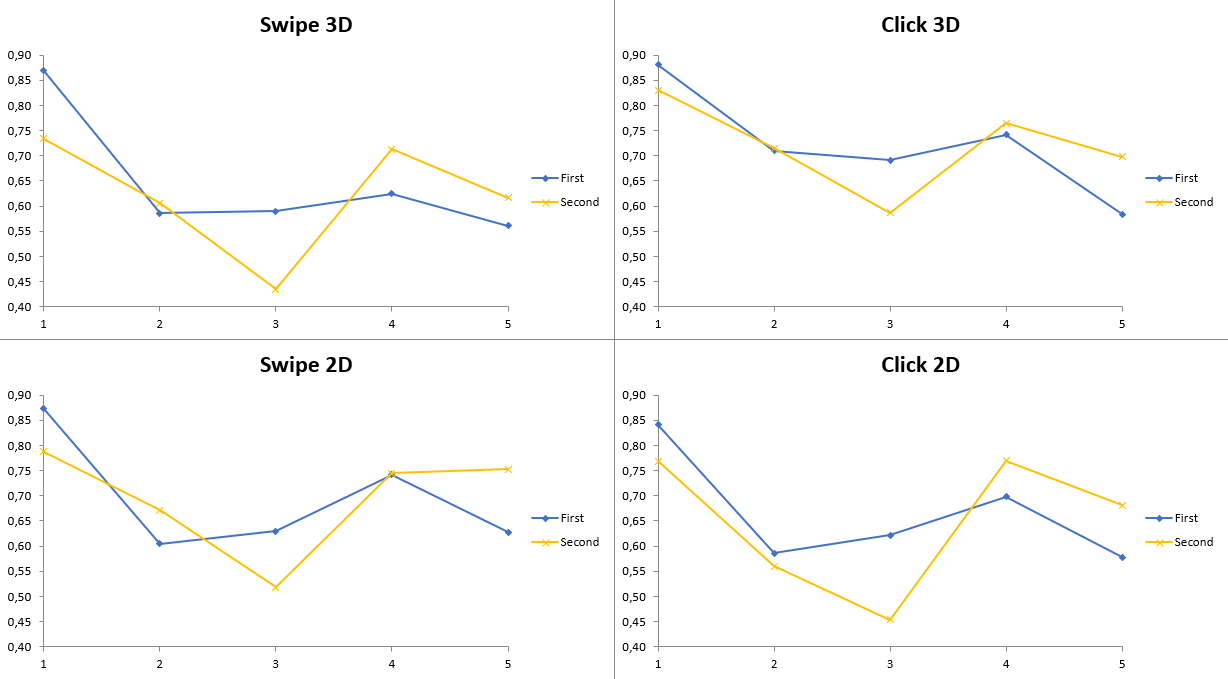
\includegraphics[width=\linewidth]{diag/ref_tThink_tAbs.png}
	\caption{Zestawienie wykresów $n_{t}$ w~zależności od poziomu dla pierwszego i~drugiego przejścia gry.}
	\label{fig:diag:ref:tThink_tAbs}
\end{figure}

Zobaczyć na nim można ciekawą zależność, która występuje we wszystkich typach interfejsów. Krzywe wyznaczone przez dane zarówno w~zakresie pierwszego przejścia gry jak i~drugiego są podobne dla każdej wersji. Widząc grę po raz pierwszy użytkownicy potrzebują względnie najwięcej czasu na zrozumienie prezentowanych im treści, bo zajmuje im to zwykle około 85\% całego czasu wykorzystanego w~trakcie przechodzenia tej planszy. Interesującym okazać się może również fakt, iż ponownemu podejściu do tego samego poziomu towarzyszyły podobne wartości $n_{t}$ (około 75\%). Podyktowane może być to faktem, iż zaimplementowany w~nim samouczek bardzo odcina się od dalszej zawartości gry, a~co za tym idzie gracze przyzwyczajeni do normalnej rozgrywki po raz kolejny muszą się dostosować do prezentowanej im treści.
Zaskakującym okazał się fakt, iż przy drugim podejściu do rozgrywki typowy użytkownik więcej czasu spędza na zastanawianiu się jak optymalnie przejść poziomy czwarty oraz piąty. Interpretować można to jako rezultat chęci poprawienia swoich wcześniejszych wyników (zostały im one przy pierwszym podejściu ukazane jako liczba zdobytych gwiazdek). Poziomy te są pierwszymi nietrywialnymi dla gracza znającego podstawowe mechaniki gry, co tłumaczyć może skok pomiędzy danymi z trzeciego oraz czwartego poziomu. \\

\subsection{Popełniane błędy}
Drugim kluczowym aspektem wpływającym na ocenę rozgrywki użytkownika są interakcje, jakie wykonał w~trakcie przechodzenia poszczególnych poziomów. Do tego grona zaliczają się zarówno zwykłe dotknięcia ekranu jak i~rotacje wykonywane na pierścieniach. Połączenie tych statystyk pozwala w~bardzo prosty sposób oszacować jak dużo użytkownicy używający tej aplikacji pozostawiają przypadkowi w~celu osiągnięcia zamierzonych celów. 

Podobnie jak w~przypadku przedstawiania danych dla absolutnego czasu, zarówno rotację jak i~kliknięcia przedstawić można w~zestawieniu z danymi referencyjnymi (tab. \ref{tab:ref_data}). w~przypadku tych statystyk również należy rozróżnić wyniki pomiędzy kategoriami Click i~Swipe. Rysunki
\ref{fig:ref:rotations} oraz \ref{fig:ref:Clicks} przedstawiają zestawienia odpowiednich wykresów dla średniej ilości rotacji i~kliknięć na poziomach. Wartym zauważenia jest, że dla tego typu danych referencja określona jest w~sposób dokładny, brak na niej odchylenia standardowego. Wynika to z faktu, iż ilość i~referencyjny sposób wykonania zadanych interakcji istnieje tylko jeden i~jest on powtarzalny dla dowolnej ilości prób.

\begin{figure}[h!]
	\centering
  	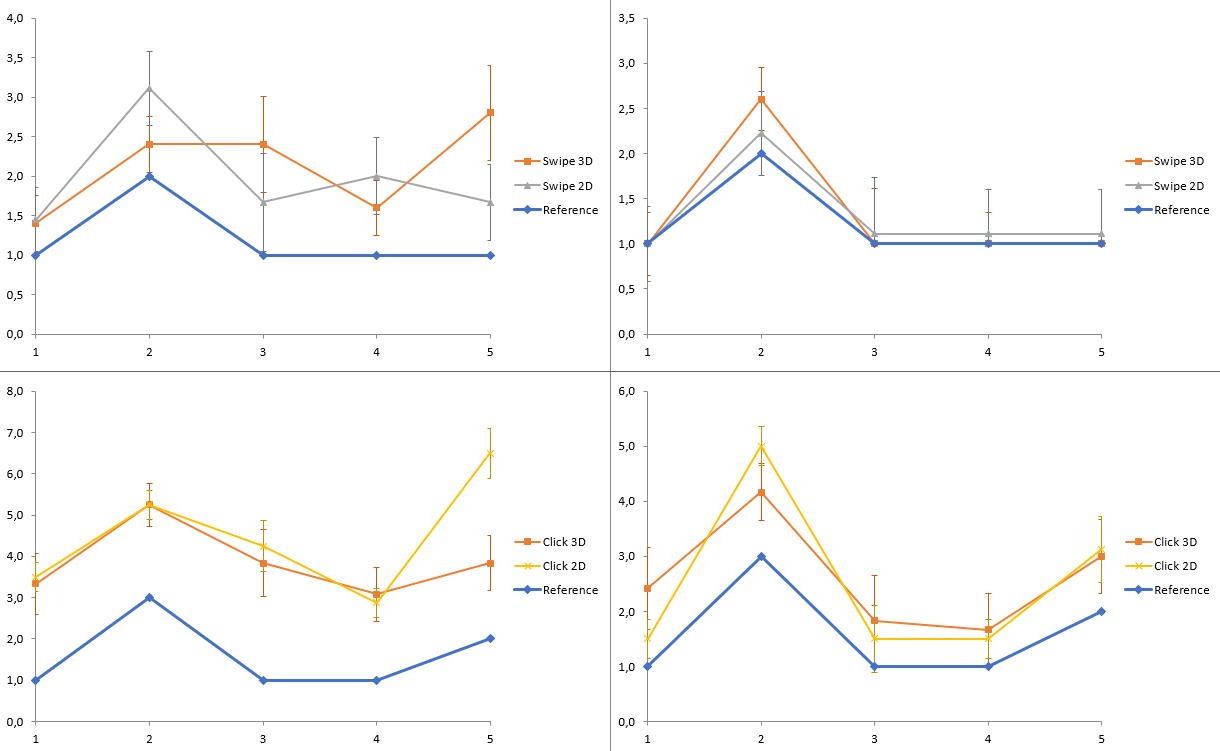
\includegraphics[width=\linewidth]{diag/ref_rotations.png}
	\caption{Wykres przedstawiający porównanie średniej ilości rotacji wykonanych dla interfejsów z dwóch kategorii do wartości referencyjnych (od lewego górnego rogu: Swipe pierwsze podejście, Swipe drugie podejście, Click pierwsze podejście, Click drugie podejście). Oś odciętych oznacza kolejne poziomy gry, podczas gdy oś rzędnych określa średnią ilość rotacji w~danej wersji gry.}
	\label{fig:ref:rotations}
\end{figure}

Analizując dane związane z wykonywanymi przez użytkowników rotacjami można zauważyć ciekawą zależność. w~przypadku interfejsów kategorii Swipe doświadczeni gracze zupełnie podświadomie wykorzystują fakt, iż licznik rotacji w~tych wersjach inkrementuje się dopiero po puszczeniu pierścienia, z którym wchodzą w~interakcję. Obracają oni nim zatem do czasu aż znajdą w~ich odczuciu najlepsze jego ułożenie, które pozwoli im na uzyskanie jak najbardziej optymalnego czasu. Objawia się to tym, że dane obliczone dla drugiego podejścia w~grach wykorzystujących te interfejsy bardzo zbliża się do wartości referencyjnych nawet na poziomie czwartym oraz piątym. Zupełnie inaczej przedstawia się to dla interfejsów Click, gdyż grając w~bardzo niewielu użytkowników zbliżyło się do wartości wyznaczonych przez twórców. Średnie ilości obrotów dla doświadczonych graczy oscylują tam w~granicach jednego obrotu więcej niż jest to przewidziane. Wnioskiem z tego może być to, iż nawet mając lepsze pojęcie o mechanikach kierujących grą i~będąc przyzwyczajonymi do sposobu interakcji dalej często popełniają błędy związane z kierunkiem, w~którym chcą żeby obrócił się dany pierścień.

Największą ilość rotacji wykonanych zaobserwować można, niezależnie od wersji gry, na poziomie drugim. Jego względnie złożony kształt, wpływa zatem na jego zrozumienie, nawet dla graczy znających już mechaniki gry. Użytkownicy na tym poziomie potrafili zbędnie obracać środkowym pierścieniem poszukując ukrytego rozwiązania, które nie istnieje na tej planszy. 

Wartym zwrócenia uwagi jest fakt, iż, z wyjątkiem pierwszego przejścia poziomu piątego, interfejsy z kategorii Click charakteryzują się podobną ilością rotacji na poziom. Oznacza to jednak tylko to, że sposób w~jaki przedstawione są informacje dodatkowe na poziomie nie wpływa na decyzje gracza związane z testowaniem różnych rozwiązań łamigłówek. \\

\begin{figure}[h!]
	\centering
  	\includegraphics[width=\linewidth]{diag/ref_Clicks.png}
	\caption{Wykres przedstawiający porównanie średniej ilości kliknięć wykonanych dla interfejsów z dwóch kategorii do wartości referencyjnych (od lewego górnego rogu: Click pierwsze podejście, Click drugie podejście, Swipe pierwsze podejście, Swipe drugie podejście). Oś odciętych oznacza kolejne poziomy gry, podczas gdy oś rzędnych określa średnią ilość rotacji w~danej wersji gry.}
	\label{fig:ref:Clicks}
\end{figure}

Podobną analizę wykonać można dla średniej ilości kliknięć wykonywanych przez użytkowników. Pierwszym wnioskiem, który wysnuć można obserwując wykresy z wynikami jest fakt, iż niezależnie od wersji oraz doświadczenia gracza wykonywanych było średnio przynajmniej dwa kliknięcia więcej niż jest to konieczne. Jest wiele czynników, które wpływać mogą na taką zależność. Najbardziej prawdopodobnym jednak wydaje się to, że elementy,  z którymi możemy wejść w~interakcję, a~zwłaszcza kulki, są zbyt małe. Zaobserwowana zostało zachowanie, że czasem, by umiejscowić sferę w~punkcie startowym użytkownicy musieli wykonywać parę podejść zanim w~końcu udało im się zakomunikować grze swoją potrzebę. Również należy pamiętać, iż z racji tego, że gra wspiera mechanikę wielokrotnego dotyku, jako kliknięcie rejestrowane był dowolny nacisk, nawet taki, który związany był z trzymaniem telefonu w~rękach i~przypadkowym dotknięciem ekranu innym palcem. 

W grze zaimplementowana została ukryta mechanika, o istnieniu której użytkownicy nie byli informowani. Pozwalała ona na przyśpieszenie początkowej animacji wczytywania poziomu, która, jak się okazało, bardzo szybko zaczynała graczy denerwować. Jej przerwanie wiąże się z dotknięciem palcem w~dowolnym miejscu ekranu, a~co za tym idzie wyjaśniać ona może zwiększone ilości tej statystyki dla doświadczonych graczy, którzy mieli już szansę samodzielnie odnaleźć tę mechanikę.

Wartym odnotowania, jest fakt, iż niezależnie od podejścia użytkowników do gry interfejsy odpowiednio z kategorii Click i~Swipe miały mniej kliknięć dla wersji 3D, niż 2D. Jest to zależność niespodziewana, gdyż wykorzystywały one pozornie dużo bardziej inwazyjny sposób przedstawienia upływu czasu. Użytkownicy jednak bardzo szybko nauczyli się nie wchodzić w~interakcję z elementami przestrzeni, które nie są kulkami i~pierścieniami. Dla wersji gry przedstawiających czas jako element interfejsu użytkownika zanotowano odwrotną zależność. Początkowo jest on ukryty i~dopiero po ustawieniu pierwszej kulki rozwija się. Nacisk na niego jeszcze przed rozpoczęciem właściwej rozgrywki również na to pozwala. Okazało się, że gracze często chcą móc oszacować jak dobre ustawienie należy znaleźć, by uzyskać trzy gwiazdki. Wpływało to oczywiście na fakt, iż doświadczony użytkownik chcąc dowiedzieć się więcej o aktualnej planszy wykonywał dodatkowy dotyk jeszcze zanim wystartowała gra.\\

Opracowane w~ten sposób dane pozwalają na względne oszacowanie jak dobrze gracze radzili sobie przy pierwszym i~drugim podejściu. Korzystając jednak ze wzoru \ref{eq_errors} jesteśmy jednak w~stanie wyznaczyć średnią ilość błędów, jakie wykonywali oni w~czasie rozgrywki. 
Na rysunku \ref{fig:diag_errors_1} przedstawiony został wykres porównujący ilość popełnianych błędów przy pierwszym przejściu gry z rozróżnieniem na poziom, na którym błędy te zostały zarejestrowane. Rysunek \ref{fig:diag_errors_2} przedstawia analogiczne dane dla drugiego podejścia, które wykonywali gracze.

\begin{figure}[h!]
	\centering
  	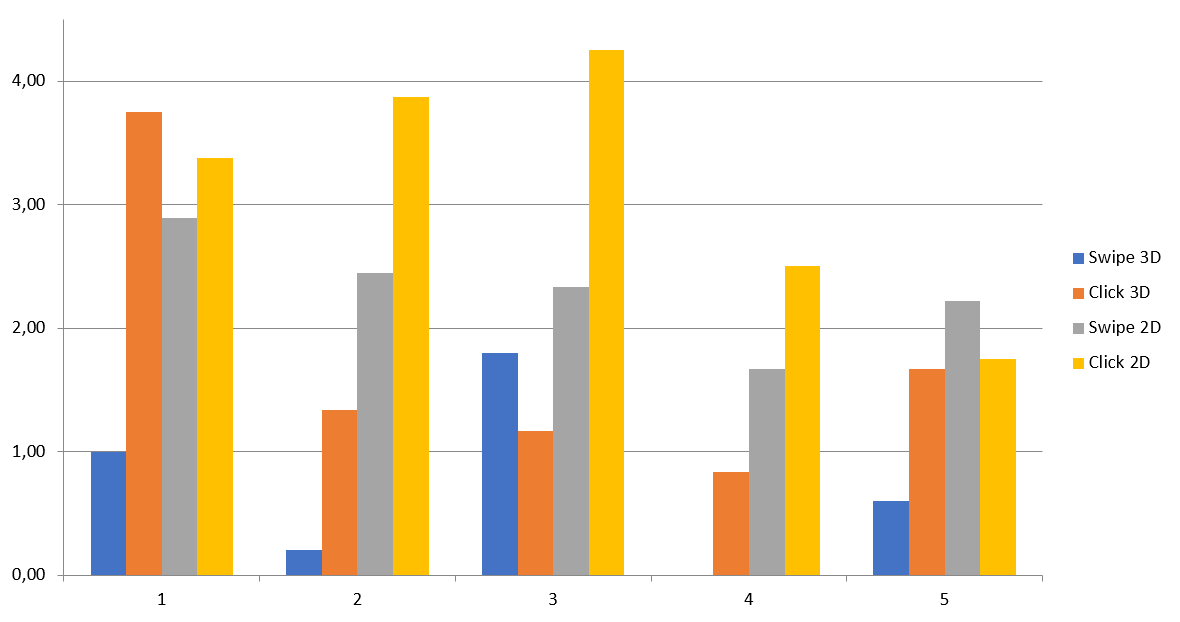
\includegraphics[width=\linewidth]{diag/errors_1.png}
	\caption{Wykres przedstawiający średnią ilość błędów popełnianych przy pierwszym przejściu gry w~zależności od poziomu. Oś odciętych oznacza kolejne poziomy gry, podczas gdy oś rzędnych określa średnią ilość błędów w~dane wersji gry.}
	\label{fig:diag_errors_1}
\end{figure}

\begin{figure}[h!]
	\centering
  	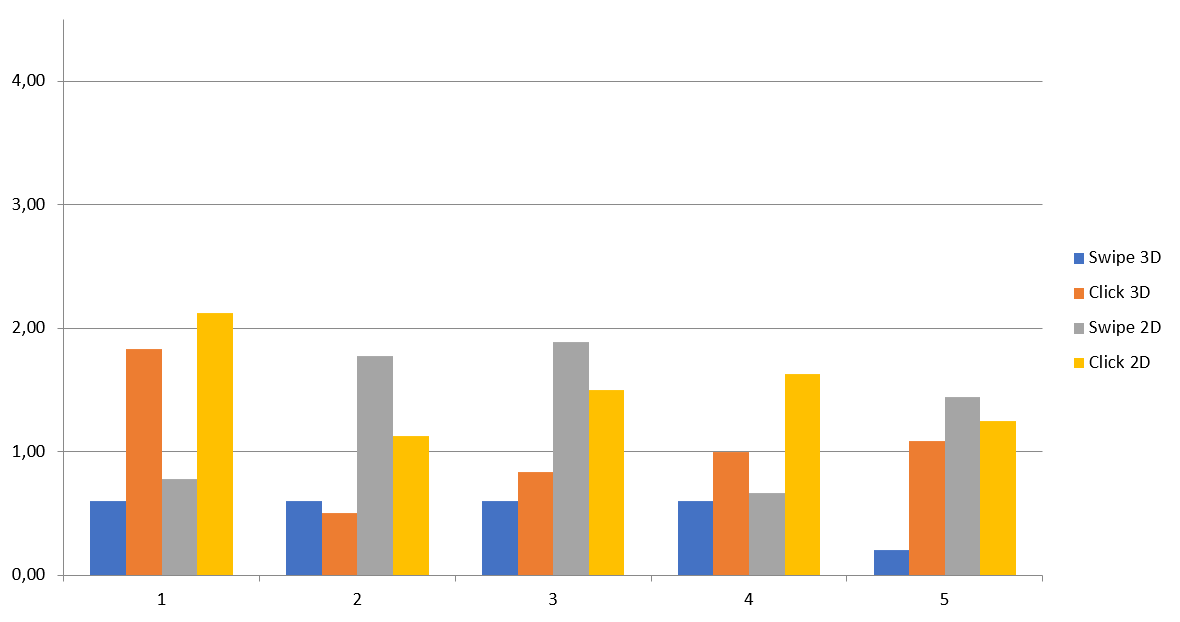
\includegraphics[width=\linewidth]{diag/errors_2.png}
	\caption{Wykres przedstawiający średnią ilość błędów popełnianych przy drugim przejściu gry w~zależności od poziomu. Oś odciętych oznacza kolejne poziomy gry, podczas gdy oś rzędnych określa średnią ilość błędów w~dane wersji gry.}
	\label{fig:diag_errors_2}
\end{figure}

Dzięki takiemu przedstawieniu danych zaobserwować można ciekawe zależności w~błędach, które popełniają użytkownicy. Jak można było się spodziewać, gracz doświadczony wykonuje ponad dwukrotnie mniej akcji, które nie są wspierane przez aplikację. 

Łatwo zauważyć, że już przy pierwszym podejściu użytkownicy popełniają ich najmniej dla wersji gry wykorzystującej interfejs Swipe 3D. Zastanawiające jest, że dla poziomu drugiego i~czwartego średnia ilość popełnionych błędów wzrosła w~drugim przejściu. Gdy gra osoba niedoświadczona to wyniki uzyskane dla tych plansz są bardzo satysfakcjonujące, gdyż oscylują one w~granicach zera. Biorąc pod uwagę wyniki zaprezentowane na rysunkach \ref{fig:ref:rotations} oraz \ref{fig:ref:Clicks} wywnioskować można że błędy te wynikają głównie z faktu niepotrzebnych dotknięć wykonanych na ekranie, które nie są związane z rotacjami pierścieni.

Dla wersji gry wykorzystującej interfejs Click 2D zarejestrowanych zostało najwięcej błędów. Jak pokazują dane przedstawione wyżej wysokie wartości w~tych wykresach spowodowane są niepotrzebnymi operacjami, do których zaliczają się zarówno zbędne dotyki jak i~obroty fragmentów labiryntu.

\subsection{Różnice pomiędzy podejściami}
Ważnym aspektem przeprowadzonych na potrzebę tej pracy badań jest porównanie sposobu, w~jaki grali użytkownicy za pierwszym i~drugim razem, gdy przechodzili te same poziomy. By lepiej je przeanalizować wykorzystane zostały dane względne, które obliczane są ze wzoru \ref{eq_relative}. Wartym do odnotowania jest że dla tego typu informacji brak jest wartości referencyjnych, gdyż każda ze zbieranych statystyk w~tym wypadku równa by była zeru. Wynika to z faktu, iż dane referencyjne zebrane zostały przez twórców rozgrywki, gdzie różnice w~przechodzeniu przez nich kolejnych poziomów są pomijalne.

Podobnie jak w~przypadku nieprzetworzonych informacji, tutaj też analizę należy rozpocząć od czasów, w~jakich udało się użytkownikom przejść poziomy. w~tym wypadku jednak uzyskanie odpowiedniej klarowności przedstawionych danych oprócz wykresu dla $t_{abs}$ umieszczono również informacje o $t_{think}$. Zestawienie tych dwóch wykresów umieszczone zostało na rysunku \ref{fig:diag:rel:mean_AbsThinkTime}. Takie podejście pozwala na zrozumienie, co było głównym czynnikiem wpływającym na takie a~nie inne wyniki całkowitego czasu potrzebnego na przejście poszczególnych poziomów.

\begin{figure}[h!]
	\centering
  	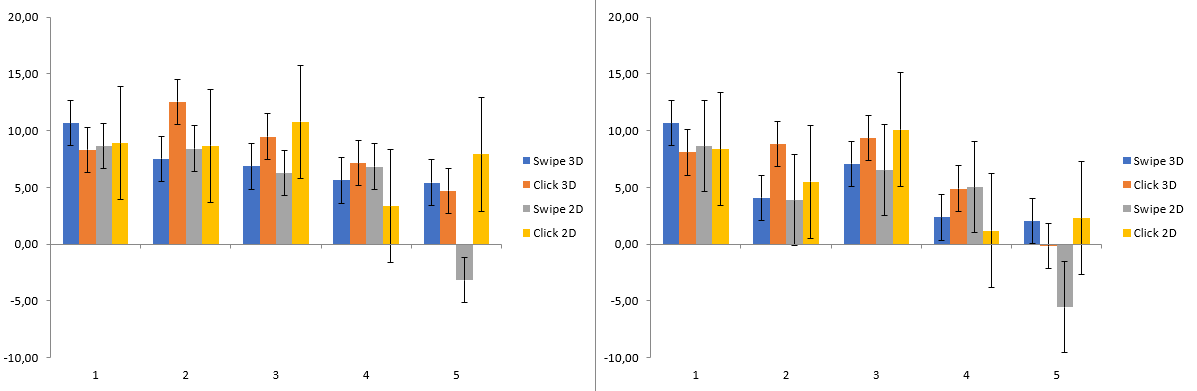
\includegraphics[width=\linewidth]{diag/rel_mean_absThinkTime.png}
	\caption{Wykresy przedstawiający średnie względne czasy przejść poziomów. Od lewej: dane dla $t_{abs}$ i~dane dla $t_{think}$. Oś odciętych oznacza kolejne poziomy, zaś rzędnych określa względny czas.}
	\label{fig:diag:rel:mean_AbsThinkTime}
\end{figure}

Przyglądając się przedstawionym danym bardzo łatwo zauważyć można duże podobieństwo między tymi dwoma wykresami. Oznacza to, że różnice w~czasie absolutnym podyktowane są głównie tym, jak długo użytkownicy zastanawiali się nad rozwiązaniem konkretnych poziomów. Statystyki względne są w~większości wypadków większe od zera, co oznacza, że zmalał czas, który potrzebny im był na etap rozgrywki. Jedynym wyjątkiem są w~tym wypadku wyniki dla piątego poziomu w~wersji Swipe 2D. Zaobserwować można tam, iż użytkownicy potrzebowali tam najwięcej czasu na namysł. Nie można jednak wykluczyć, iż wynik jednostki zakrzywił te wyniki. Zastąpienie wartości średniej medianą (rys. \ref{fig:diag:rel:median_AbsThinkTime}) pozwolił na odsiew danych brzegowych. Dzięki temu stwierdzić można, iż wynik dla poziomu piątego faktycznie został zakrzywiony. Wartym odnotowania również jest fakt, iż wartości mediany są w~podobnej zależności względem siebie co te ze średniej. Zestawienie ze sobą tych danych pozwala na lepsze zrozumienie rozłożenia wyników.

\begin{figure}[h!]
	\centering
  	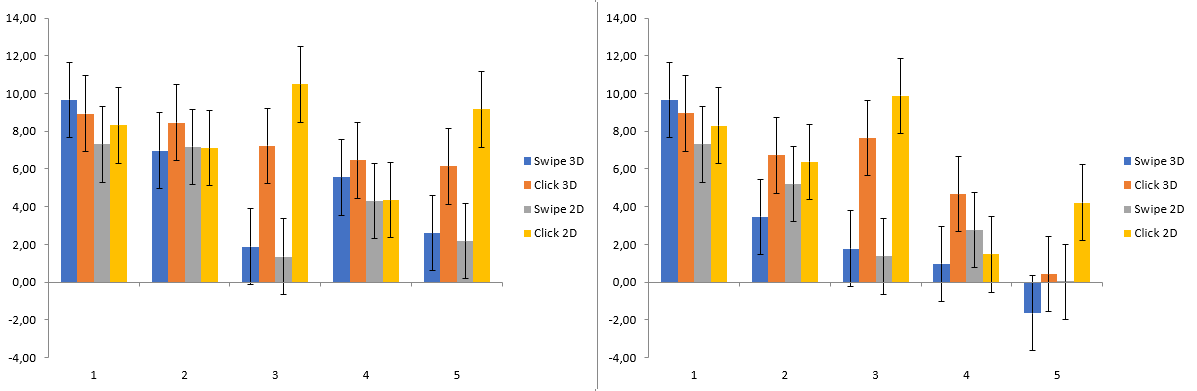
\includegraphics[width=\linewidth]{diag/rel_median_absThinkTime.png}
	\caption{Wykresy przedstawiający medianę z względnych czasów przejść poziomów. Od lewej: dane dla $t_{abs}$ i~dane dla $t_{think}$. Oś odciętych oznacza kolejne poziomy, zaś rzędnych określa względny czas.}
	\label{fig:diag:rel:median_AbsThinkTime}
\end{figure}

Analizując zebrane wyniki zobaczyć można, iż wraz ze zwiększaniem się numeru poziomu, wartości względne czasu zbliżają się do zera. Wynika to z tego, że grając użytkownicy zdobywają coraz to większe doświadczenie. Wraz z nim mniej czasu potrzebują na zastanawianie się w~ramach danego poziomu jakie akcje są dla nich dozwolone. Dla dalszych poziomów czas ten zależy jedynie od trudności samego labiryntu, a~nie stopnia, w~jakim zrozumiana jest gra. Po dłuższej rozgrywce spodziewać się zatem można, że wartości względne w~dalszych poziomach będą bardzo zbliżone do 0.

Na poziomach pierwszym i~drugim użytkownicy zanotować można największe różnice w~zastanawianiu się nad ruchem (czasy względne są dla nich największe). Każdy z nich zawiera w~sobie samouczki, które zmieniają na pewien czas sposób rozgrywki. Drastyczne zmniejszenie czasu spędzonego na kontemplacje i~próby zrozumienia przedstawionych treści dla poziomu pierwszego jest proste do wytłumczenia. Doświadczony gracz szybciej jest w~stanie zrozumieć bądź przypomnieć sobie sposób w~jaki aplikacja przekazuje informacje odnośnie akcji, które gracz musi wykonać. Dysponując tą wiedzą szybko są oni w~stanie je przeprowadzić i~jednocześnie rozwiązać znajdującą się na tej planszy trywialną wersję labiryntu. Złożoność poziomu trzeciego polega na tym, że w~trakcie ruchu kulki, gdzie gracz nie spodziewa się żadnych zaskoczeń, następuje przybliżenie kamery na skrzyżowanie do którego dochodzi właśnie sfera. Zdarzenie to występuje jednak dopiero po wystartowaniu gry, stąd też użytkownicy, którzy wiedzą, że to się wydarzy nie potrzebują zastanawiać się nad znalezieniem rozwiązania innego niż to, które jest im od początku proponowane.\\

Podobną analizę przeprowadzić można dla danych względnych dotyczących średnich obrotów pierścieni oraz dotknięć ekranu, które wykonywali użytkownicy. Wykresy przedstawiające obliczone wartości dla tych statystyk zobaczyć można na rysunkach \ref{fig:diag:rel:mean_Rotations} - \ref{fig:diag:rel:mean_Clicks}.

\begin{figure}[h!]
	\centering
  	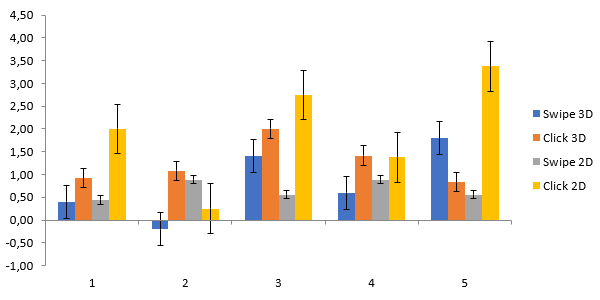
\includegraphics[width=0.9\linewidth]{diag/rel_mean_rotations.png}
	\caption{Wykres przedstawiający średnie względne rotacje wykonane na poziomach. Oś odciętych oznacza kolejne poziomy, zaś rzędnych określa względny czas.}
	\label{fig:diag:rel:mean_Rotations}
\end{figure}

Obserwując dane zebrane o względnych rotacjach zobaczyć można, iż dla interfejsu Swipe 2D zanotowano sumarycznie najmniejsze wartości względnych rotacji. Oznacza to, że użytkownicy nie za pierwszym i~za drugim razem wykonywali podobną ilość obrotów pierścieni przy rozgrywaniu poziomów. Nie należy jednak zapominać, iż interakcja w~interfejsach kategorii Swipe pozwala na "przytrzymywanie" elementów planszy. Oznacza to, że kąt $\alpha_r$ zanotowanego pojedynczego obrotu opisać tam można zależnością $\alpha_r = n * 90$, gdzie n jest dowolną liczbą całkowitą. Inaczej sprawa wygląda dla interfejsów Click, gdyż tam n wynosić może tylko +/-1. Z tego powodu spodziewać się można, iż część użytkowników korzystała z tej zależności i~zastanawiając się nad prawidłowym ułożeniem pierścieni po prostu ustawiała je w~coraz to kolejnych obrotach nie przestając przy tym ich przytrzymywać, co poskutkowało mniejszą ilością wynikowych obrotów. \\
Zastanawiającym jest, że pomimo tego faktu wyniki Swipe 3D dla drugiego poziomu wskazują na to, że część użytkowników wykonała więcej obrotów za drugim przejściem (uwidocznione to zostało ujemną wartością względną dla tych danych). Szybkie porównanie z wartościami z tabeli \ref{tab:analysis_Swipe3d} pozwala na określenie, że proceder ten powtórzył się dla prawie 75\% wszystkich użytkowników, którzy korzystali z wersji gry wykorzystującej ten interfejs (trzeci kwartyl wartości względnej jest ujemny). Dopatrywać się tu zatem można, iż użytkownicy odnosili wrażenie, iż ukryte jest w~ramach tego poziomu ustawienie pierścieni, które pozwala na szybsze jego przejście. \\
Zaskakujące również okazać się może to, że dla interfejsu Click 2D - dla którego to w~większości przypadków odnotowano największe wartości względne - poziom drugi okazał się tym, w~którym ilości rotacji za pierwszym i~drugim przejściem niemalże się pokrywały. Wynikać to może z faktu iż ograniczenia, które niesie ze sobą ta wersja gry wpływają na to, czy gracz ma ochotę szukać bardziej optymalnego rozwiązania dla względnie oczywistego poziomu.

\begin{figure}[h!]
	\centering
  	\includegraphics[width=0.9\linewidth]{diag/rel_mean_Clicks.png}
	\caption{Wykres przedstawiający średnie względne ilości kliknięć wykonane na poziomach. Oś odciętych oznacza kolejne poziomy, zaś rzędnych określa względny czas.}
	\label{fig:diag:rel:mean_Clicks}
\end{figure}

W przypadku względnych dotyków ekranu zaobserwować można, że dla każdego poziomu gry wykorzystującej interfejs Click 2D różnica w~ich ilości pomiędzy pierwszym a~drugim podejściem danego użytkownika jest największa. Na tej podstawie stwierdzić można, że to zestawienie heurystyk przyczynić się mogło do największej ilości niepotrzebnych kliknięć. Największy skok odnotowany został w~trzecim poziomie, gdzie doświadczony użytkownik wykonywał przeszło 6 operacji mniej. Przyczyną tego zarejestrowanego zachowania może być wspomniane już wcześniej zabranie kontroli jakie ma miejsce w~samouczku na tej planszy. Gracze nie wiedząc co się dzieje starają się szybko zareagować na wyświetlaną im animacje. Przy pierwszym podejściu nie wiedzą oni, że nie jest wymagane od nich wykonanie żadnej akcji, więc próbują jak najlepiej odnieść się do tego, co postrzegają jako zmienianie się reguł gry.
Inaczej prezentuje się ta sytuacja dla doświadczonych użytkowników, którzy w~tej sytuacji nie próbują już wykonywać żadnych dodatkowych operacji. Jako potwierdzenie tej teorii wyznaczyć można to, że dla tej planszy zanotowana została największa ilość kliknięć w~wersji gry Swipe 3D, którą pod względem spełnianych heurystyk określić można jako przeciwieństwo wcześniej wspomnianej Click 2D.

Do przemyśleń skłania fakt, iż dla drugiej wersji gry korzystającej z interfejsów kategorii Swipe nie została zaobserwowana tak drastyczna zmiana pomiędzy wersjami jak ta opisana wyżej. Tylko dla pierwszych dwóch poziomów względna różnica w~ilości dotyków plasowała się na drugim miejscu w~kategorii ilości a~i~to o niewielką ilość. Oznaczać to może, iż fakt, iż wersja ta prezentowała niektóre części interfejsu w~przestrzeni gry mogło mieć pozytywny wpływ na zrozumienie gry już za pierwszym razem.

Najbardziej zbliżonymi do oczekiwanych wyników odznaczyła się wersja gry spełniająca obie heurystyki, czyli Swipe 2D. Jej wyniki nie były najmniejsze dla każdego poziomu, ale brak w~niej gwałtownych skoków, które oznaczać mogą zagubienie użytkownika przy pierwszej rozgrywce i~różnice w~ilości kliknięć na planszę są na względnie tym samym poziomie przez cały czas. Spodziewać by się można, że zależność ta zachowana jest również dla dalszej części gry.\\

Należy pamiętać, że ilość interakcji wymaganych w~celu osiągnięcia tego samego celu dla interfejsów typu Click i~Swipe jest różna. Żeby móc lepiej przeanalizować te dane należy sprowadzić je do porównywalnego stanu. Z tego też powodu zostały one podzielone przez referencyjne minimalne ilości wymaganych interakcji, które przedstawione zostały w~tabeli \ref{tab:ref_data}. Dane przekształcone w~ten sposób zestawione zostały ze swoimi nieznormalizowanymi wersjami (rys. \ref{fig:diag:rel:mean_RotationsNorm} - \ref{fig:diag:rel:mean_ClicksNorm}).

W tak przekształconych danych zmniejszone zostało przekłamanie związane z poziomem drugim oraz piątym, w~których to wykonać trzeba większą ilość operacji obrotu by osiągnąć taki sam obrót końcowy pierścieni (dla gier korzystających z interfejsu Swipe). Wynika to z faktu, iż mechanika klikania pozwala tylko na obrót o 90 stopni podczas gdy przeciąganie palcem do zadanego obrotu nie zawiera tego ograniczenia. 

\begin{figure}[h!]
	\centering
  	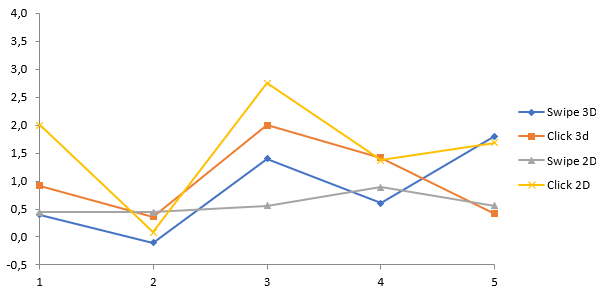
\includegraphics[width=\linewidth]{diag/rel_mean_rotationsNorm.png}
	\caption{Zestawienie wykresów przedstawiających względne ilości rotacji (od lewej: dla danych nieznormalizowanych oraz dane znormalizowanych). Oś odciętych oznacza kolejne poziomy, zaś rzędnych określa względne rotacje.}
	\label{fig:diag:rel:mean_RotationsNorm}
\end{figure}

Znormalizowanie danych dla obrotów pierścieni dla interfejsów Swipe wpływa tylko na dane z poziomu drugiego. Inaczej wygląda to dla interfejsów Click, gdzie dla niektórych poziomów należy wykonać tych obrotów więcej, by osiągnąć ten sam efekt. Skutek przekształcenia tych danych zaobserwować można na podstawie zależności pomiędzy interfejsem Click 3D a~Swipe 2D. Okazuje się bowiem, iż średnia ilość względnych rotacji porównywanie większa jest w~tej wersji gry wykorzystującej interakcje w~postaci przeciągania. Pomniejszony został również odnotowany wcześniej skok w~tej statystyce dla piątej planszy w~Click 2D. Okazało się, iż jest ona porównywalna do tego co zaprezentowane zostało w~Swipe 3D.

\begin{figure}[h!]
	\centering
  	\includegraphics[width=\linewidth]{diag/rel_mean_ClicksNorm.png}
	\caption{Zestawienie wykresów przedstawiających względne ilości kliknięć (od lewej: dla danych nieznormalizowanych oraz dane znormalizowanych). Oś odciętych oznacza kolejne poziomy, zaś rzędnych określa względne kliknięcia.}
	\label{fig:diag:rel:mean_ClicksNorm}
\end{figure}
W wypadku ilości dotknięć ekranu zaobserwować można większe zmiany w~zależnościach pomiędzy poszczególnymi wynikami. Okazuje się tutaj bowiem, że wyniki interfejsu Click 3D są korzystniejsze aniżeli wcześniej uznane za najlepsze dane ze Swipe 2D. Dla poziomu drugiego oraz piątego okazało się bowiem, że są one najbliższe zeru. Duże skoki widoczne w~nieznormalizowanej wersji Click 2D również zostały zniwelowane. Jedynym miejscem, dla którego interfejs ten przedstawia największą liczbę względnych dotknięć ekranu jest poziom trzeci.
Uwidoczniona została nieregularność wyników dla Swipe 3D. Tylko tam na podstawie zebranych danych brak jest możliwości określenia, jak zmieniać by się mógł ten wykres dla dalszych części gry.

Kategorie Click i~Swipe są do siebie o wiele bardziej porównywalne dzięki wykonaniu operacji normalizowania. Wszystkie wyniki są bardziej zbliżone między sobą a~co za tym idzie bardziej uwydatnione zostały zależności pomiędzy określonymi wersjami gry.

%CHAPTER___________________________________________________________________________________________________
\chapter{Podsumowanie}

W przedstawionej pracy wykonane zostało badanie mające na celu sprawdzenie, czy ogólnie przyjęte heurystyki dotyczące użyteczności mają wpływ na zrozumienie gry przez użytkowników. Wysnute zostały trzy hipotezy, których spełnienie bezpośrednio potwierdziłoby zadaną tezę. w~rozdziale tym sprawdzone zostanie, które z przyjętych w~drugim rozdziale pracy domniemań udało się potwierdzić przeprowadzonymi testami.

\section{Hipoteza I}
\textit{Zrozumienie mechanik gry mobilnej przychodzi użytkownikom łatwiej dla gier spełniających więcej heurystyk użyteczności.}\\

Zrozumienie mechanik gry zbadane zostało w~tej pracy poprzez porównanie wyników graczy niedoświadczonych z tymi wygenerowanymi przez te same osoby, ale kiedy mają już one pojęcie o tym, jak gra działa. Poprzez porównywanie graczy z samymi sobą zminimalizowane zostały czynniki, takie jak predyspozycje jednostki, czy jej umiejętność rozwiązywania problemów. 
Najlepsze zrozumienie mechanik rozpoznać można zatem za pomocą danych względnych, które przedstawione zostały na rysunkach \ref{fig:diag:rel:mean_AbsThinkTime} - \ref{fig:diag:rel:mean_ClicksNorm}. Najmniejsze różnice w~danych zebranych dla nowicjusza a~tą samą osobą zaznajomioną ze sposobem w~jaki działa aplikacja oznaczać zatem mają najlepsze poznanie mechanik już przy pierwszym podejściu.\\

Wersja gry wykorzystująca interfejs Swipe 2D spełnia przedstawione warunki zarówno dla czasu absolutnego, jak i~dla ilości wykonanych rotacji w~ramach poziomu. w~przypadku danych niepoddanych operacji normalizowania (rys. \ref{fig:diag:rel:mean_Clicks}) spełnione one zostały również dla ilości dotyków ekranu wykonywanych na planszach. w~przypadku znormalizowania informacji ta wersja aplikacji okazuje się nie spełniać zadanych założeń.

Zrozumiane zostało w~niej najszybciej co jest celem gry i~jak można wchodzić w~interakcję z elementami na planszy. w~zestawieniu z interfejsami z kategorii Click okazało się jednak iż stosunkowo wykonano w~tym procesie więcej niepotrzebnych dotknięć. Znormalizowane dane umniejszają jednak pojedyncze błędy takie jak przypadkowe muśnięcie ekranu innym palcem w~znacznie większym stopniu dla wersji gry wykorzystujących klikanie jako podstawowy sposób interakcji. 

Rozumiejąc znaczenie tej zależności stwierdzić jednak można, iż Swipe 2D okazał się wersją gry, która pozwala na najszybsze zrozumienie mechanik rozgrywki. Z racji tego, że to właśnie on spełniał obydwie z wybranych heurystyk stwierdzić można, iż ta hipoteza została potwierdzona.

\section{Hipoteza II}

\textit{Użytkownicy popełniają mniej błędów w~wypadku gier spełniających więcej heurystyk użyteczności}\\

Łatwo można zidentyfikować poprawność tej hipotezy poprzez analizę wykresu przedstawionego na rysunku \ref{fig:diag_errors_sum}. Przedstawia on sumaryczne średnie ilości błędów uzależnione od wersji gry i~podejścia do rozgrywki graczy.

\begin{figure}[h!]
	\centering
  	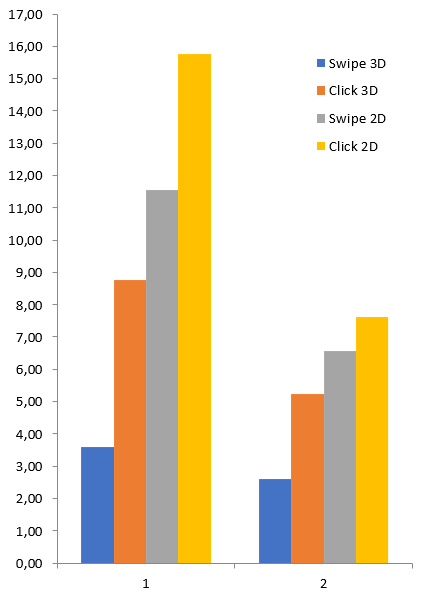
\includegraphics[width=7cm]{diag/errors_sum.png}
	\caption{Wykres przedstawiający sumaryczne średnie ilości błędów popełnianych przez graczy w~zależności od tego, które jest to ich podejście do przechodzenia zadanych poziomów. Oś odciętych oznacza numery kolejnych prób, podczas gdy oś rzędnych określa sumaryczną średnią ilość błędów w~dane wersji gry.}
	\label{fig:diag_errors_sum}
\end{figure}

Zauważyć można, iż zależności pomiędzy sumarycznymi średnimi ilościami błędów popełnianych w~różnych wersjach gry niezależna jest od tego jak dobrze użytkownicy znają mechaniki gry. Zarówno w~przypadku pierwszego jak i~drugiego podejścia zachowane zostały proporcje w~jakich popełniane są błędy. Zaskakującym okazało się, że wersja gry Swipe 2D, czyli ta, która spełnia obie zadane heurystyki jest na drugim miejscu w~kwestii średniej ilości popełnianych błędów na poziomach. Interfejs, który w~założeniu wygenerować miał najwięcej niepożądanych interakcji - Click 3D - okazał się od niego pod tym względem bardziej optymalnym. 

Wersje aplikacji, które spełniały tylko pierwszą bądź drugą heurystykę okazały się najbardziej skrajnymi w~badanej kwestii - Click 2D (spełniona pierwsza heurystyka) zarejestrował najwięcej błędów podczas gdy Swipe 3D (spełniona druga heurystyka) najmniej. 
Osiągnięcie takich wyników pozwala na poddanie pod wątpliwość, czy samo spełnianie bądź też nie wybranych zasad projektowania dotyczących użyteczności może mieć wpływ na to, jak dużo nieprzewidzianych zachowań wykonają użytkownicy. Z tej racji druga z wysnutych hipotez nie mogła zostać potwierdzona.

\section{Hipoteza III}
\textit{Użytkownicy grający w~grę spełniającą mniej heurystyk użyteczności osiągają gorsze wyniki od tych, którzy grają w~wersję spełniającą ich więcej.}\\

W niejednej grze bardzo trudne jest określenie co definiuje jakość z jaką udaje się graczowi wykonywać zadania. w~przypadku badanej aplikacji pod uwagę brany został czynnik, który w~niej samej stanowi wyznacznik tego ile gwiazdek, czyli nagrody za przejście poziomu, udzielić użytkownikowi. Jedyną statystyką, która na to wpływa jest czas, w~jakim udało się przejść dany poziom. w~zebranych na potrzeby tej pracy danych opisywana była ona jako $t_abs$. Minimalny czas, w~jakim można przejść daną planszę, od wystartowania rozgrywki do dostarczenia ostatniej kulki do środka labiryntu, jest niezależny od rodzaju interfejsu użytkownika. 

Dla każdego poziomu zdefiniowana jest wartość referencyjna, której użytkownicy nie są w~stanie przekroczyć. Zebrane wyniki pomniejszyć można zatem o referencje zyskując tym samym informację o tym jak optymalne drogi zostały wybrane dla poszczególnych wersji gry. Na rysunku \ref{fig:diag_tball_sum} przedstawiony został wykres, na którym zamieszczone zostały te sumaryczne średnie wartości nadmiaru wykorzystanego czasu na przejście poziomu dla pierwszego i~drugiego przejścia gry. Jako odchylenie standardowe przyjęte zostały sumy odchyleń dla poszczególnych poziomów i wersji gry, które zamieszczone zostały w~tabelach \ref{tab:results_Swipe3d} - \ref{tab:analysis_Click2d}.\\

\begin{figure}[h!]
	\centering
  	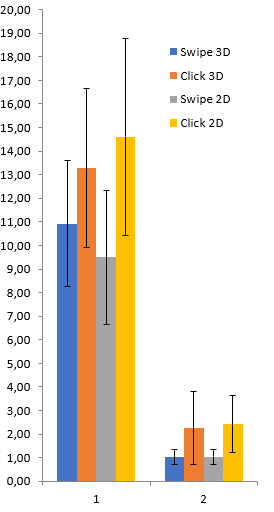
\includegraphics[width=7cm]{diag/tBall_sum.png}
	\caption{Wykres przedstawiający sumaryczny średni nadmiar czasu $t_{ball}$ w~zależności od numeru przejścia zadanych poziomów. Oś odciętych oznacza numery kolejnych prób, podczas gdy oś rzędnych określa sumaryczną średni czas osiągnięty w~danej wersji gry.}
	\label{fig:diag_tball_sum}
\end{figure}

Zaobserwować można, że dla wyników zdefiniowanych w~opisany powyżej sposób najlepsze zostały osiągnięte dla wersji Swipe 2D. Dla doświadczonych użytkowników wyniki te plasują się na podobnym poziomie co dla drugiego interfejsu z tej samej kategorii - Swipe 3D. Podobną zależność można zaobserwować dla tych dwóch aplikacji, które korzystają z interakcji kliknięć. Tak jak przy pierwszym podejściu wyraźnie lepszy jest Click 3D, to przy drugim granica ta się zaciera. Widoczne rozróżnienie pozostaje jednak między kategoriami, co pozwala na określenie iż sposób, w~jaki wymagany jest wykonywanie podstawowych interakcji w~grze ma wpływ na wynik, który zostanie uzyskany. Wersja spełniająca obie heursytyki okazała się tą, na której gracze byli w~stanie osiągnąć najlepsze czasy dla plansz. Oznacza to, iż trzecia hipoteza została potwierdzona.


%CHAPTER___________________________________________________________________________________________________
\chapter{Wnioski}

W pracy udało się udowodnić dwie z trzech postawionych hipotez. Mimo tego, że zaprojektowanymi badaniami nie udało się potwierdzić prawdziwości drugiej z nich to zauważony został wpływ spełniania heurystyk użyteczności na zrozumienie rozgrywki przez użytkowników. Interfejs Swipe 2D okazał się pod wieloma względami najlepszym w przedstawianiu graczom abstrakcyjnych zadań, które mieli oni wykonać. Nie w każdym jednak przypadku testowym udało się uzyskać wartości, które jednoznacznie pokazałyby, iż wersja niespełniająca żadnej z wybranych zasad okazałaby się najgorsza. \\

Doszukiwać się można wielu czynników, które miały na to wpływ. Najważniejszym okazał się jednak fakt, iż projekt przycisku używany w interfejsach Click 2D oraz Swipe 2D był mniej czytelny aniżeli przekazywanie informacji w przestrzeni gry. Przedstawiony w ten sposób czasomierz wyglądał jak każdy inny przycisk, które to gracze mogli naciskać w celach takich jak np. zatrzymanie rozgrywki na jakiś czas. Z tego też powodu intuicyjnym wydawało się im, że również i za tym elementem kryła się jakaś przydatna funkcjonalność.
Przycisk ten wymagał dodatkowej interakcji by przed rozpoczęciem gry gracze mogli dowiedzieć się informacji, która przedstawiona w postaci siatek w grze znajdowała się tam przez cały czas. Sam fakt iż element ten reagował na akcje ze strony gracza bardzo istotnie wpłynął na ilość zarejestrowanych błędów, dla wersji gry, które go wykorzystywały. Po naciśnięciu go w momencie, gdy faktyczna gra jeszcze się nie rozpoczęła, wyświetla on animację, która polega na rozwinięciu schowanego wcześniej paska czasomierza. \\
Uznać można, iż niewłaściwym zachowaniem ze strony projektowej było traktowanie dotyku elementów dwuwymiarowego interfejsu jak każdego innego nacisku na ekran. Z drugiej strony, wyłączenie elementów znajdujących się w tej przestrzeni z badań mogłoby wpłynąć na niezarejestrowanie zachowania ze strony użytkowników, które mogłoby zostać uznane za nieprawidłowe.\\
Innym czynnikiem, który miał duży wpływ na zebrane wyniki było udzielenie zbyt dużej swobody osobom biorącym udział w badaniu. Przez to, że dopiero przed drugim podejściem do gry dowiadywali się, że biorą udział w eksperymencie zaobserwowano dużą różnicę w swobodzie ich zachowań względem przejść. Przechodząc zadane poziomy po raz pierwszy użytkownicy dużo więcej czasu potrafili spędzić nieskupieni na grze, którą testowali. Ich wzrok częściej uciekał do osoby nadzorującej badanie, potrafili również zapomnieć na chwilę o wykonywanych zadaniach wdając się w wymianę zdań z towarzyszącymi im osobami. Gdy wiedzieli o tym, że ich wyniki są rejestrowane, dużo sumienniej podchodzili do rozgrywki. Zależność ta mogła mieć wpływ na różnicę pomiędzy wynikami dla początkujących i doświadczonych graczy. Z racji tego, że nie odnotowano jednak, by dla którejś wersji gry było to zjawisko bardziej intensywne niż dla innych, to założyć można, iż nie miało ono wpływu na relacje pomiędzy uzyskanymi danymi.\\
Warunki, w których przeprowadzane były badania potrafiły być bardzo zmienne. Nawet w ramach pokazów na jednym z wydarzeń oscylować mogły one od bardzo niekorzystnych po takie, w których trudno o jakiekolwiek rozproszenie z zewnątrz. Testowanie w takich środowiskach miało na celu symulację warunków, w których użytkownicy używają smartfonów. Doszukiwać się można jednak, iż z racji tego, że brak było wpływu na to, kiedy i jak zmieniały się te warunki, to mogły mieć one niejednolicie niekorzystny wpływ na wyniki wygenerowane dla poszczególnych wersji gry.\\
Mimo przedstawionych ograniczeń i błędów w projekcie badania zarejestrowane zostały wyraźne różnice pomiędzy przygotowanymi wersjami gry. Zebrane dane nie wyglądają na dzieło przypadku, dostrzec można w nich zależności związane z wybranymi heurystykami użyteczności. Gdy sposób interakcji w grze wydaje się graczom nieintuicyjny to wykonują oni więcej niepotrzebnych akcji. Niezrozumienie wybranych elementów interfejsu, które spowodowane może być przykładowo ich niespójnością również generuje niepożądane zachowania wśród graczy. Fakt, iż zebrane wyniki pomagają w dojściu do takich wniosków traktowane jest jako wyznacznik, iż wersje gry zostały między sobą wystarczająco rozróżnione. \\


W przyszłych badaniach rozważyć można by było opracowanie szerszego zakresu heurystyk. Pozwoliłoby to na określenie odpowiednich wag dla poszczególnych zasad projektowania użyteczności w grach. Przetestowanie większej ich ilości należałoby jednak przygotować w inny sposób, niż przedstawiony w tej pracy, gdyż wiązałoby się to ze znacznym zwiększeniem ilości przygotowanych wersji gry. Chcąc przetestować wszystkie kombinacje dla n heurystyk potrzeba by było stworzyć $2^{n}$ spełniających je aplikacji. Badania poszerzyć można by było również o zastosowanie techniki przeglądu ekspertów w celu potwierdzenia, czy zasady, które wybrane zostały dla danej wersji aplikacji są faktycznie w niej spełniane.\\
Poszerzyć można by również zakres badanych informacji o takie, które zbierane by były za pomocą urządzenia do śledzenia wzroku użytkownika (eng. \textit{eye-tracker}). Dane zebrane w ten sposób przyczynić by się mogły do lepszego określenia zachowań użytkowników podczas gry \cite{online_Eyetracking}. Dzięki temu lepiej można by ocenić takie aspekty jak to, co przyczynia się do największej ilości popełnianych błędów w danej grze.\\
Podczas drugiego przechodzenia gry użytkownicy w pewnym stopniu pamiętali, jakie akcje wykonywali na poziomach i jak one wyglądały. Wpływało to na szybkość zrozumienia przez nich przedstawianych im informacji, gdyż już wcześniej musieli oni wykonać ten proces. W przyszłości zminimalizować można tą zależność poprzez wizualną zmianę prezentowanych labiryntów między przejściami. Nie miało by to w żadnym stopniu wpływać na sposób rozwiązywania poziomów, a jedynie przedstawić ten sam labirynt w innej kolorystyce i ułożeniu początkowym.\\


Podsumowując, w pracy tej udało się znaleźć związek pomiędzy zasadami określającymi użyteczność gry, a zrozumieniem jej mechanik przez użytkowników. Przeprowadzone badania potwierdziły, że gracze szybciej są w stanie zrozumieć nierzadko abstrakcyjne zadania postawione im przez aplikację w momencie, gdy spełnia ona odpowiednie heurystyki. Temat nie został jednak wyczerpany i projektowanie przyszłych doświadczeń w tej dziedzinie mogło by się przyczynić również do ulepszenia i większego sprecyzowania ogólnie przyjętych zasad projektowania gier.



%CHAPTER___________________________________________________________________________________________________
\chapter{Abstract}


More and more usability heuristics are emerging from year to year, aimed at defining a set of rules that must be met in order to create an user-friendly product. They cover wide range of computer programs - from most basic interactive applications to even more specific case of mobile games. However, it is difficult to determine how much of an impact they have on the actual quality of the player's gameplay. For the purpose of this work, it has been checked whether the use of PLAY usability heuristics has a positive effect on understanding the previously unknown mechanics of a mobile game.

A study was carried out for this purpose, in which an unique puzzle game was prepared in four versions that met a different set of selected design principles. Subjects were divided into appropriate subgroups without distinguishing them by age or gender. Each user had to pass five initial levels twice. Selected app utilizes unique rules and requires from the user to perform abstract tasks in order to proceed. Players that took part in this experiment has never before seen such game mechanics and therefore in their first attemt thay had to learn them from scratch. After users were finished with the initial levels they were told to play the game some more allowing them to properly learn how it works. When they gained proper skills they were asked to start it again from first level. Thanks to this approach it was managed to get results for one player, while he was both a novice and a person who knows well the rules of the game. This way, the impact of the individual's predisposition has been minimized on the final test results.

From the analysis of those results it was proved that the version of the game that fulfilled the most of the PLAY heuristics was also the most understandable for the players. It has also been confirmed that players achieve worse results in games where less intuitive interactions are used to perform basic operations.

\pagenumbering{gobble}
\bibliography{biblio} 
%\bibliographystyle{unsrt}
\bibliographystyle{ieeetr}
\renewcommand{\listoffigures}{\begingroup
\tocchapter
\tocfile{\listfigurename}{lof}
\endgroup}
\listoffigures
\chapter{Zawartość płyty}
\begin{enumerate}[label={[\arabic*]}]
  \item Tekst pracy w~formacie PDF
  \item Pliki z wynikami przeprowadzonych badań
  \item Plik z wynikami przeprowadzonej analizy
\end{enumerate}

\end{document}